\documentclass[UTF8,a4paper,zihao=-4,fontset=windows]{ctexart}
\usepackage[margin=2.5cm]{geometry}
\usepackage{amsmath,amssymb,graphicx,booktabs,array,adjustbox,caption,float,needspace,longtable}
\usepackage[unicode,hidelinks,hypertexnames=false]{hyperref}
\usepackage{fancyhdr}
\usepackage{tikz}
\usetikzlibrary{arrows.meta,positioning}
\setmainfont{Times New Roman}
\setlength{\parindent}{2em}
\linespread{1.16}
\setlength{\parskip}{0pt}
\setlength{\abovedisplayskip}{7pt}
\setlength{\belowdisplayskip}{7pt}
\setlength{\textfloatsep}{9pt}
\setlength{\intextsep}{9pt}
\captionsetup{font=small,labelfont=bf,textfont=bf,labelsep=space,justification=centering,singlelinecheck=false}
\captionsetup[table]{position=bottom,skip=5pt}
\captionsetup[figure]{position=bottom,skip=5pt}
\newcommand{\figtabnote}[1]{\par\vspace{3pt}{\fontsize{9}{11}\selectfont\raggedright\noindent 注：#1\par}}
\ctexset{section={format=\Large\heiti,beforeskip=12pt,afterskip=6pt},subsection={format=\large\heiti,beforeskip=9pt,afterskip=5pt}}
\pagestyle{fancy}\fancyhf{}\fancyfoot[C]{\thepage}\renewcommand{\headrulewidth}{0pt}
\setlength{\headheight}{14pt}
\setcounter{secnumdepth}{0}
\emergencystretch=2em
\begin{document}
\begin{center}{\zihao{2}\heiti 基于残差场景与滚动调整的微网购电及储能调控策略}\end{center}
\begin{center}\large\bfseries 摘\quad 要\end{center}
针对光伏出力、负载及电价变化下的微网购电问题，考虑日前预测难以覆盖日内偏差，建立由确定性线性规划、残差场景随机规划和日内滚动调整组成的调控模型。在满足逐时供电与储能约束的基础上，区分计划购电、计划调整和紧急购电三类费用，并以实际运行轨迹评价策略。
\par
针对问题一，将一天划分为144个10分钟时段，以储能侧充放电量为变量，建立含日初日末储电量相等约束的线性规划。求得全天购电量59482.70 kWh，费用35101.57元；储电量在1200—10800 kWh内变化。容量与功率的121组组合试验表明，所考察范围内费用为35056.72—40319.54元。
\par
针对问题二，采用最近同类型日预测负载、最近五日预测光伏，以最近十日配对残差构建场景，形成共同日前计划及场景补救决策。实际运行采用受储电量和功率约束的充放电规则。在2月1日至12月31日的334天内，总费用为1370.17万元，紧急购电量为12.79万kWh。
\par
针对问题三，按历史误差组合外部光伏预报与历史预测，在6、12、18时更新剩余时段购电计划。完整追索式方案费用为1326.66万元，较问题二降低3.18\%，紧急购电量减少83.46\%。消融试验中，仅在12、18时调整的方案费用最低，为1315.58万元，但紧急购电量较主方案增加，说明更新频次应结合费用和应急需求选择。
\par
针对问题四，利用历史同类型日电价和当日已观测电价预测未来价格，以实际电价结算。日前方案与滚动方案费用分别为1440.18万元和1395.35万元，后者节约3.11\%。保持日均电价的五种波动情形中，滚动方案节约率由1.17\%增至4.76\%。结果表明，储能调度与日内调整能够降低统计期费用和紧急购电量，更新时点的选择则需兼顾两项指标。
\par
\textbf{关键词：}微网调控；残差场景；两阶段随机规划；滚动优化；储能调度
\par
\clearpage
\section{1 问题重述与分析}
\subsection{1.1 研究任务}
微网通过光伏、储能和外网购电共同满足小区负载。储能可以将低价时段的电量转移至高价时段，也可吸收暂时过剩的光伏电量，但其容量、功率和能量损耗限制了转移能力。问题的关键是提前购买多少电、何时调整承诺，以及预测偏差出现后如何调度储能。
\par
问题一给出固定电价、负载和一天的光伏预测，要求在0时确定全天计划，且日末储电量回到日初水平。问题二引入实际负载和光伏变化，普通购电按计划量付费，供电不足须以五倍现货电价紧急购电。问题三增加每日四次光伏预报，允许付费调整原计划，需判断额外预报是否值得使用。问题四进一步考虑实时电价波动，重新计算日前方案和滚动方案。各问均需给出题面指定日期、时段的购电与储能结果。
\par
\subsection{1.2 方法选择与研究思路}
微网与主电网的经济协调属于能量管理层问题，区别于电压、频率等快速控制问题[1]。题目未提供线路阻抗或节点结构，因此本文以10分钟电量平衡建模，不引入无法识别参数的交流潮流方程。
\par
问题一的费用和储能动态均为线性关系，线性规划可直接处理144个时段的耦合。问题二具有“先承诺、后补救”的决策顺序，采用两阶段随机规划[2]：历史残差场景保留多条偏差路径，场景平均费用对应购电费用目标，比单点预测更充分地描述不确定性，也避免按所有最坏情形安排购电。
\par
问题三采用滚动优化：新信息到达后重新求解未来部分，已经执行的部分保持不变。该思路已有微网能量管理研究支持[3]。本文只调整购电与储能，不增加机组启停等整数决策。预测与权重选择均按时间先后进行，仅使用决策时刻以前的信息，遵循时间序列预测的滚动评价原则[4]。问题四保持原有供电模型，只扩展价格预测及结算，便于比较新增价格信息的作用。
\par
各问采用SciPy线性规划接口[5]与HiGHS求解器，稀疏约束结构适合修正单纯形等线性规划方法[6]。图1概括四问从确定性计划到预报、价格驱动调整的递进关系。
\par
\begin{figure}[H]\centering
\begin{tikzpicture}[box/.style={draw,rounded corners=2pt,text width=3.35cm,minimum height=1.0cm,align=center,font=\small},>=Stealth]
\node[box] (a) at (0,0) {问题一\\确定性线性规划};
\node[box] (b) at (4,0) {问题二\\残差场景日前规划};
\node[box] (c) at (8,0) {问题三\\预报组合与滚动调整};
\node[box] (d) at (12,0) {问题四\\因果价格预测};
\draw[->] (a)--(b);\draw[->] (b)--(c);\draw[->] (c)--(d);
\node[draw,rounded corners=2pt,align=center,text width=11.6cm,font=\small] (e) at (8,-1.55) {历史信息生成预测与场景\quad{}→\quad{}因果执行\quad{}→\quad{}按实际电价结算};
\draw[->] (b.south)--(4,-.9)--(e.north -| b.south);
\draw[->] (c.south)--(e.north);
\draw[->] (d.south)--(12,-.9)--(e.north -| d.south);
\end{tikzpicture}
\caption{四问的模型递进与共同评价流程}
\figtabnote{历史信息生成预测与场景，实际运行后再计算费用。}
\end{figure}
\section{2 数据整理与建模假设}
\subsection{2.1 数据来源和时间对齐}
附件1提供144个时段的电价、负载与光伏预测功率；附件2提供2025年365天的实际负载和光伏功率；附件3每天有0、6、12、18时四次预报，每次包含未来24个整点的光伏功率；附件4给出365天的实际电价。数值区域检查未发现缺失或负值，因此未对原始功率与价格做异常值删除或平滑处理。附件3的合并日期单元格按同日四次预报补齐日期标签，保留其数值不变。
\par
设一天共有$N=144$个时段，时段$t=0,\ldots,143$对应区间$[t\Delta,(t+1)\Delta)$，其中$\Delta=1/6$小时。源表00:10和24:00分别为首、末时段的右端点；题面10:00—10:10对应数组下标60。功率统一转换为时段电量：
\par
\begin{equation}
L_{i,t}=P^L_{i,t}\Delta,\qquad G_{i,t}=P^G_{i,t}\Delta. \tag{1}
\end{equation}
仿真从1月1日以6000 kWh开始连续运行，1月份用于形成历史预测与运行状态；按结果模板要求，费用及策略比较统计2月1日至12月31日，共334天。下文“统计期”均指这334天。2月1日的储电量继承1月31日运行结果，并不重置为6000 kWh。
\par
\subsection{2.2 建模假设及适用范围}
（1）将微网作为单节点能量系统，以10分钟电量平衡描述供需关系；忽略线路损耗、通信时延和电压约束，储能损耗由效率参数计入。
\par
（2）充电效率和放电效率分别取0.9，即一次完整充放电的能量效率为0.81。储能不考虑自放电、寿命衰减和随荷电状态变化的效率，5000 kW功率上限在每个10分钟时段内恒定。
\par
（3）微网不向外网售电，超过负载且无法存储的电量计为余电。问题二至四允许紧急购电补足缺口，外网供电容量按无限制处理。
\par
（4）按附件的负载模式，将周五、周六归为低负载类，其余日期归为另一类；用决策时已获得的近期同类样本预测负载。
\par
（5）问题三以0时原计划为调整结算基准，减购部分保留原价的50\%作为违约费用；增购部分按原价的1.5倍支付。多次修订只结算各时段最终执行的版本，避免把同一时段反复修改的差额重复收费。问题四另外假设未来实际电价在决策时未知，预测电价用于优化，实际电价用于结算。
\par
（6）问题一以储能侧电量定义充放电变量及5000 kW上限，问题二至四以微网侧电量定义变量及上限。两种计量约定的换算见第4节；各问结果按其对应边界解释。
\par
\section{3 符号说明与公共约束}
\begin{table}[H]\centering
\fontsize{9.5}{12}\selectfont\setlength{\tabcolsep}{4pt}\renewcommand{\arraystretch}{1.12}
\begin{adjustbox}{max width=\linewidth}\begin{tabular}{lcc}\toprule
\textbf{符号} & \textbf{含义} & \textbf{单位}\\\midrule
$i,t,k$ & 日期、时段及场景下标 & —\\
$N,\Delta,K$ & 日时段数、时长及场景数：144、1/6、10 & —、h、—\\
$P^L,P^G$ & 负载功率、光伏功率 & kW\\
$L,G$ & 时段负载电量、光伏电量 & kWh\\
$g^0,g^{\tau},g^{\mathrm{fin}}$ & 原计划、更新计划、最终计划购电量 & kWh\\
$c,d$ & 问题二至四的微网侧充电量、放电量 & kWh\\
$\bar c,\bar d$ & 问题一的储能侧充电量、放电量 & kWh\\
$S$ & 储能设备内部存储电量 & kWh\\
$e,z$ & 紧急购电量、未使用余电量 & kWh\\
$r,x$ & 相对原计划的减购量、增购量 & kWh\\
$\pi,\widehat\pi$ & 实际交易电价、预测电价 & 元/kWh\\
$\eta,E_{\max}$ & 单向效率0.9、时段能量上限833.3333 & —、kWh\\
$v,\epsilon$ & 终端储电价值0.42、吞吐引导系数0.001 & 元/kWh\\
\bottomrule\end{tabular}\end{adjustbox}
\caption{主要符号与单位}
\end{table}
表中功率用于预测，电量用于优化与结算。日期下标$i$在单日模型中省略；上标$k$表示场景，上标0表示0时原计划，上标$\tau$表示在时段$\tau$开始时作出的更新。预测量用帽号表示。
\par
对问题二至四，功率上限对应时段电量上限$E_{\max}=5000\Delta=833.3333$ kWh。实际调度满足
\par
\begin{equation}
g_t+G_t+d_t+e_t=L_t+c_t+z_t,\qquad S_{t+1}=S_t+\eta c_t-d_t/\eta, \tag{2}
\end{equation}
\begin{equation}
1200\le S_t\le10800,\quad 0\le c_t,d_t\le E_{\max},\quad g_t,e_t,z_t\ge0. \tag{3}
\end{equation}
其中$z_t$为光伏富余与未使用计划购电的合计电量。将其单列后，式（2）同时描述负载供给、储能交换及余电处置。
\par
规划模型使用较窄的未来储电范围$1500\le S_t^k\le10500$，两端各保留300 kWh安全裕度；日初实测状态仍服从物理范围1200—10800 kWh。实际运行允许使用该裕度。问题二至四不施加每日首末储电量相等约束，而以$S_{i+1,0}=S_{i,144}$连接相邻日期。
\par
\section{4 问题一：确定性日前购电模型}
\subsection{4.1 线性规划的建立与求解}
对给定负载和光伏预测，决定每个时段购电量$g_t$以及储能侧充、放电量$\bar c_t,\bar d_t$，使全天费用最小：
\par
\begin{equation}
\min C_1=\sum_{t=0}^{143}\pi_tg_t. \tag{4}
\end{equation}
储能侧充入$\bar c_t$需要微网提供$\bar c_t/\eta$，储能侧放出$\bar d_t$只能向微网供给$\eta\bar d_t$，故有
\par
\begin{equation}
g_t+G_t+\eta\bar d_t=L_t+\bar c_t/\eta,\qquad S_{t+1}=S_t+\bar c_t-\bar d_t. \tag{5}
\end{equation}
\begin{equation}
\begin{gathered}
0\le\bar c_t,\bar d_t\le833.3333,\qquad g_t\ge0,\\
1200\le S_t\le10800,\qquad S_0=S_{144}=6000.
\end{gathered} \tag{6}
\end{equation}
该线性规划包含577个连续变量和290个等式约束。HiGHS返回最优状态，得到式（4）—（6）的全局最优解。
\par
按微网侧换算，$c_t=\bar c_t/\eta$、$d_t=\eta\bar d_t$，上限分别为925.9259和750.0000 kWh，即5555.56和4500.00 kW。以下问题一结果统一按储能侧列示。
\par
\subsection{4.2 购电计划与储能运行}
按题面表1、表2的格式，以下分别列出指定时段购电量、全天费用与储能充放电结果。
\par
\begin{table}[H]\centering
\fontsize{9.5}{12}\selectfont\setlength{\tabcolsep}{4pt}\renewcommand{\arraystretch}{1.12}
\begin{adjustbox}{max width=\linewidth}\begin{tabular}{lccccc}\toprule
\textbf{时间段} & \shortstack{\textbf{购电量}\\{\normalfont （kWh）}} & \textbf{时间段} & \shortstack{\textbf{购电量}\\{\normalfont （kWh）}} & \textbf{时间段} & \shortstack{\textbf{购电量}\\{\normalfont （kWh）}}\\\midrule
10:00-10:10 & 0.00 & 12:00-12:10 & 573.01 & 14:00-14:10 & 0.00\\
16:00-16:10 & 445.43 & 18:00-18:10 & 531.89 & 20:00-20:10 & 0.00\\
全天购电量 & 59482.70 & 全天购电费/元 & 35101.57 & 计量单位 & kWh、元\\
\bottomrule\end{tabular}\end{adjustbox}
\caption{问题一指定时段购电量及全天费用}
\end{table}
\begin{table}[H]\centering
\fontsize{9.5}{12}\selectfont\setlength{\tabcolsep}{4pt}\renewcommand{\arraystretch}{1.12}
\begin{adjustbox}{max width=\linewidth}\begin{tabular}{lccccc}\toprule
\textbf{时间段} & \textbf{充电量} & \textbf{放电量} & \textbf{时间段} & \textbf{充电量} & \textbf{放电量}\\\midrule
0:00-4:00 & 3966.67 & 0.00 & 4:00-8:00 & 833.33 & 7073.16\\
8:00-12:00 & 3975.83 & 1892.22 & 12:00-16:00 & 5090.76 & 101.22\\
16:00-20:00 & 0.00 & 6422.37 & 20:00-24:00 & 4800.00 & 3177.63\\
0:00储电量 & 6000.00 & — & 24:00储电量 & 6000.00 & —\\
\bottomrule\end{tabular}\end{adjustbox}
\caption{问题一储能侧充放电及首末储电量（kWh）}
\end{table}
图2中，储能在低价时段及光伏富余时充电，在较高电价及负载缺口出现时放电，日末恢复至6000 kWh。全天储能侧累计充、放电量均为18666.60 kWh；四小时窗口内的正充电量与正放电量来自不同时段的切换。
\par
\begin{figure}[H]\centering
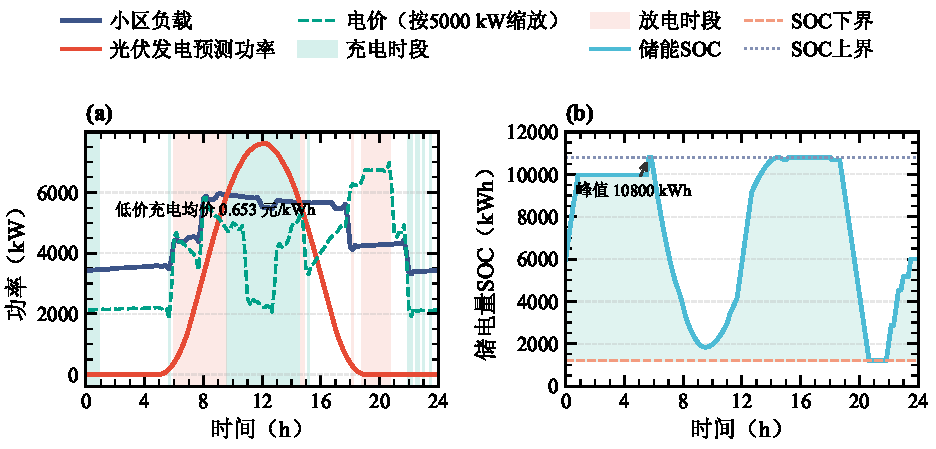
\includegraphics[width=.96\linewidth,height=7.0cm,keepaspectratio]{../new_figures_main/Q1_F1_optimal_dispatch.pdf}
\caption{问题一供需曲线与储能调控轨迹}
\figtabnote{电价按5000 kW缩放；SOC表示储能内部电量。}
\end{figure}
\begin{figure}[H]\centering
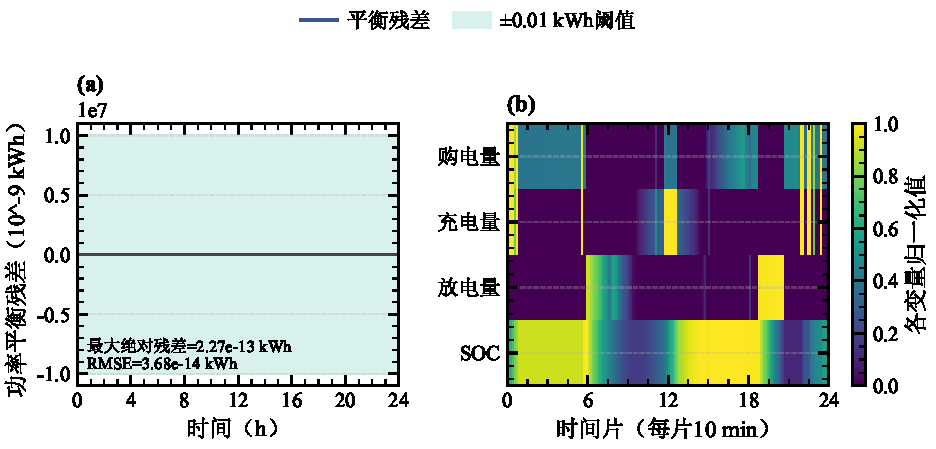
\includegraphics[width=.96\linewidth,height=7.0cm,keepaspectratio]{../new_figures_main/Q1_F2_solution_diagnostics.pdf}
\caption{问题一电量平衡与运行状态}
\figtabnote{右图对每个变量分别归一化，颜色用于比较该变量的时序变化。}
\end{figure}
图3中，最大绝对电量平衡残差为$2.27\times10^{-13}$ kWh，RMSE为$3.68\times10^{-14}$ kWh。归一化热力图中充电、放电的高值区分离，与日内储电量的上升、下降相对应。
\par
\subsection{4.3 容量与功率灵敏度}
以6000 kWh为中心，将可用储电区间写成$[6000-4800a,6000+4800a]$，其中$a=0.50,0.55,\ldots,1.00$；储能侧功率上限乘以系数$b$，取0.40、0.48、0.56、0.64、0.72、0.80、0.88、0.96、1.00、1.10、1.20。图4汇总121组容量窗口与功率系数组合的费用。
\par
\begin{figure}[H]\centering
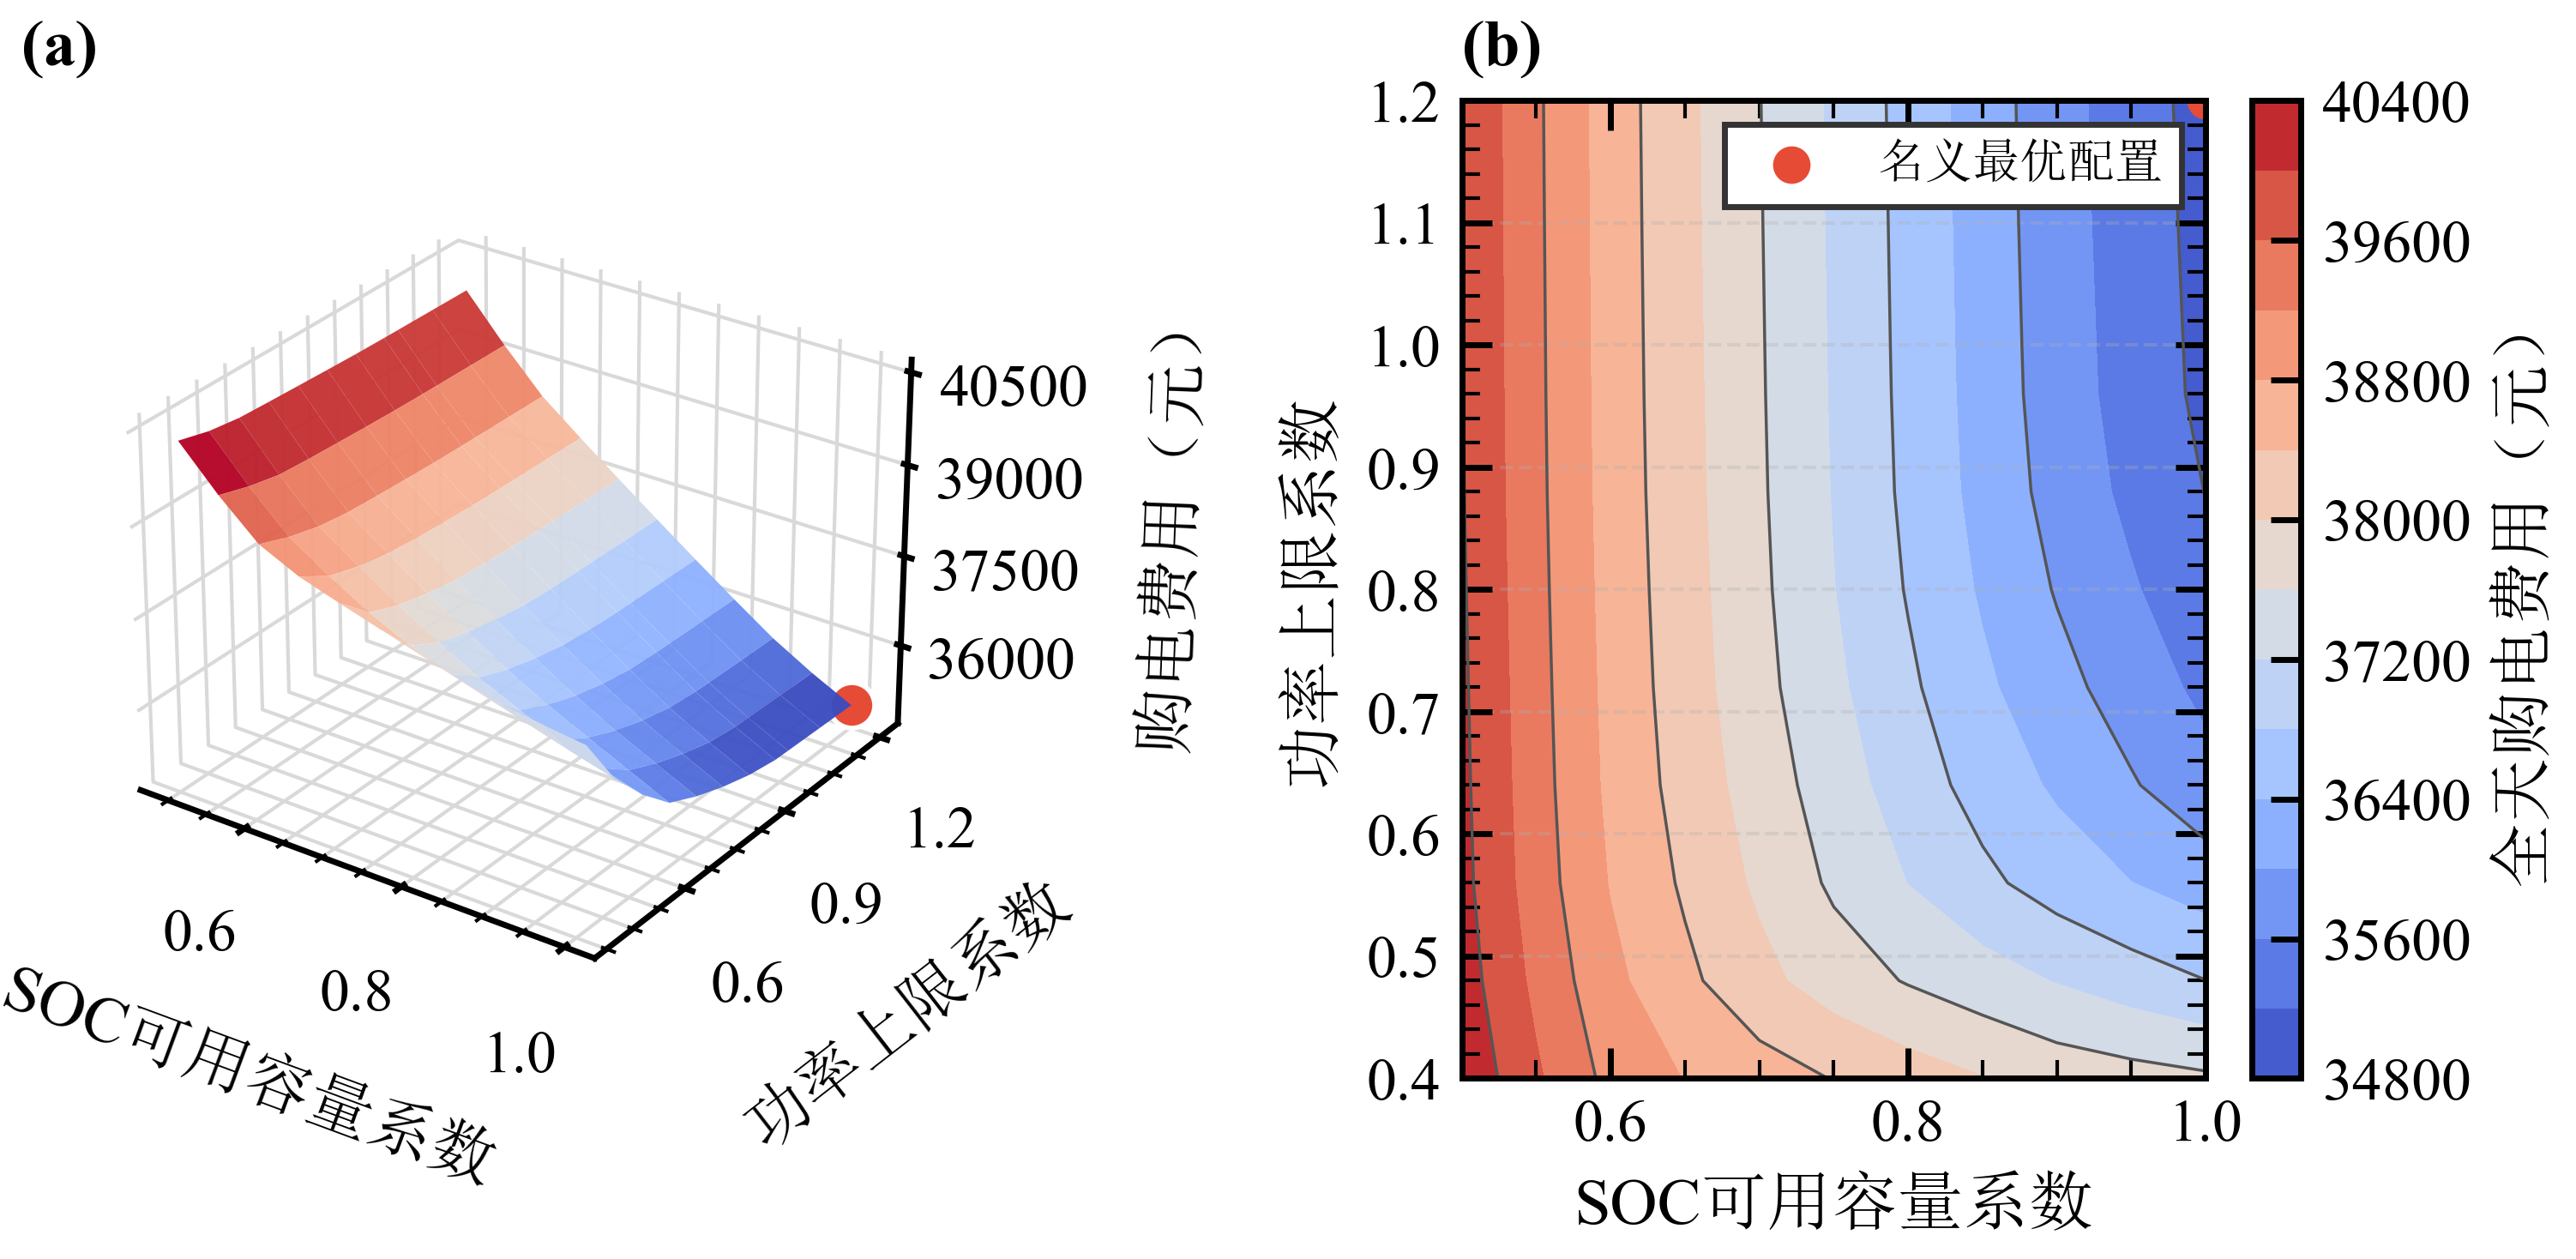
\includegraphics[width=.96\linewidth,height=7.5cm,keepaspectratio]{../new_figures_main/Q1_F3_storage_sensitivity.png}
\caption{可用储电窗口与功率上限对购电费的影响}
\figtabnote{容量系数缩放以6000 kWh为中心的可用窗口；图中标记为所测参数网格的最低费用配置。}
\end{figure}
图4的等高线在高容量区域随功率系数增加逐渐稀疏，说明此处提高功率上限的边际节约减小。网格最低费用为35056.72元，比原参数减少44.84元；扩大可用容量窗口的影响更明显。费用随边界放宽不升，与线性规划可行域扩大的关系一致。
\par
\section{5 问题二：残差场景下的日前购电与实际调度}
\subsection{5.1 点预测和配对残差场景}
负载预测取最近三个同类型日的均值，光伏预测取最近五日均值，分别记为$\widehat P^L_{i,t}$和$\widehat P^G_{i,t}$。历史不足时使用已有样本；每个历史日的残差由当时可生成的预测与实际观测之差得到。
\par
从最近十个历史日期取配对的负载与光伏残差，形成$K=10$个等权场景：
\par
\begin{equation}
\begin{aligned}
L^k_{i,t}&=\Delta\,[\widehat P^L_{i,t}+\varepsilon^L_{h_k,t}]_+,\\
G^k_{i,t}&=\Delta\,[\widehat P^G_{i,t}+\varepsilon^G_{h_k,t}]_+,
\end{aligned}\qquad [x]_+=\max(x,0). \tag{7}
\end{equation}
同一场景的负载与光伏残差来自同一个历史日，以保留二者的共同变化及全天时序形态；生成的功率经非负截断后转为电量。图5中，2025-09-23实际净负荷落在十条场景P10—P90经验分位带内的时段占79.2\%，部分午间和晚间偏差仍超出该范围。
\par
\begin{figure}[H]\centering
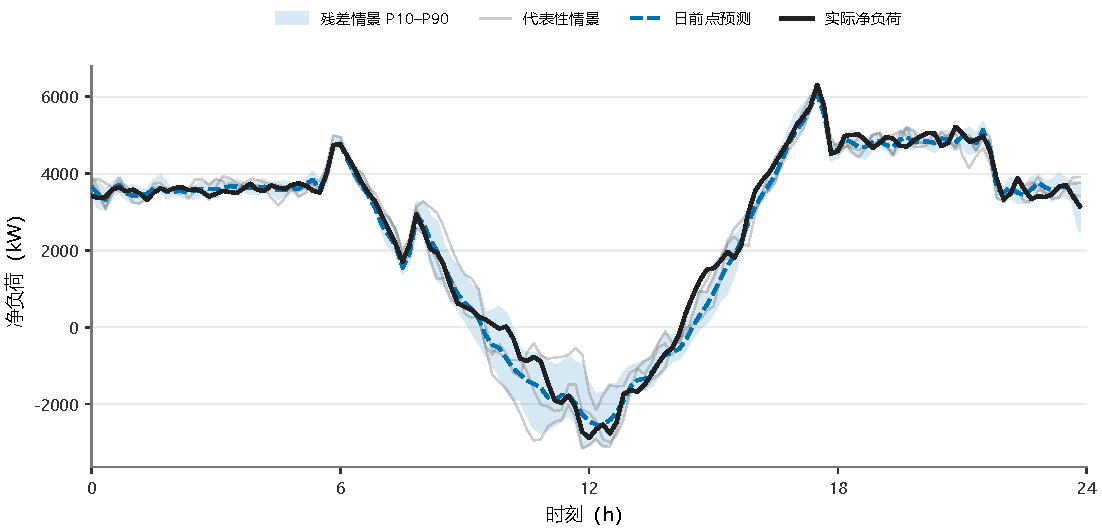
\includegraphics[width=.96\linewidth,height=6.5cm,keepaspectratio]{../new_figures_main/Q2_F2_uncertainty_scenarios.pdf}
\caption{典型日净负荷预测与历史残差场景}
\figtabnote{阴影为十条场景的P10—P90经验分位带；净负荷为负载减光伏。}
\end{figure}
\subsection{5.2 两阶段随机线性规划}
第一阶段确定所有场景共用的购电计划$g_t$；第二阶段分别安排场景下的充放电、紧急购电和余电。以场景平均运行代价评价第一阶段计划：
\par
\begin{equation}
\min\;\sum_t\pi_tg_t+\frac1K\sum_{k=1}^K\left[5\sum_t\pi_te_t^k+\epsilon\sum_t(c_t^k+d_t^k)-vS_{144}^k\right]. \tag{8}
\end{equation}
约束为各场景的式（2）、式（3）及未来规划储电范围1500—10500 kWh，其中$\epsilon=0.001$元/kWh，$v=0.42$元/kWh。吞吐惩罚抑制无经济价值的循环，终端储电价值减轻日末过度放电；二者仅用于优化引导，实际购电费按式（11）结算。
\par
第二阶段以完整场景路径安排补救，形成两阶段近似。实际运行逐时获得信息，并按下一节的储能规则执行；费用与紧急购电量均从实际轨迹汇总。
\par
\subsection{5.3 因果运行规则与结算}
每个时段先接收实际负载和光伏，计算计划购电后的净缺口$R_t=L_t-G_t-g_t$。若$R_t\ge0$，优先用可用储能补足，剩余部分紧急购买：
\par
\begin{equation}
d_t=\min\{R_t,E_{\max},\eta(S_t-1200)\},\quad e_t=R_t-d_t,\quad c_t=z_t=0. \tag{9}
\end{equation}
若$R_t<0$，先在功率和容量范围内充电，其余计为余电：
\par
\begin{equation}
c_t=\min\{-R_t,E_{\max},(10800-S_t)/\eta\},\quad z_t=-R_t-c_t,\quad d_t=e_t=0. \tag{10}
\end{equation}
更新$S_{t+1}$后进入下一时段。该规则按缺口符号选择充电或放电，从执行机制上避免同一时段同时充放电。日末状态传入下一日。实际费用为
\par
\begin{equation}
C_2=\sum_{i,t}\pi_tg_{i,t}+5\sum_{i,t}\pi_te_{i,t}. \tag{11}
\end{equation}
普通购电按计划量收费，计划电量即使转为余电，也不从第一项扣除。模型通过较高的紧急购电代价与过量计划的支出之间的权衡，形成购电承诺。
\par
\subsection{5.4 统计期结果与典型日结果}
统计期计划购电费为1292.56万元，紧急购电费为77.61万元，合计1370.17万元；紧急购电量12.79万kWh，发生于107天。负载预测MAE、RMSE分别为137.31、189.83 kW，光伏分别为151.52、304.47 kW。光伏RMSE明显较大，提示少数较大预测偏差对应较强的运行压力。
\par
\begin{figure}[H]\centering
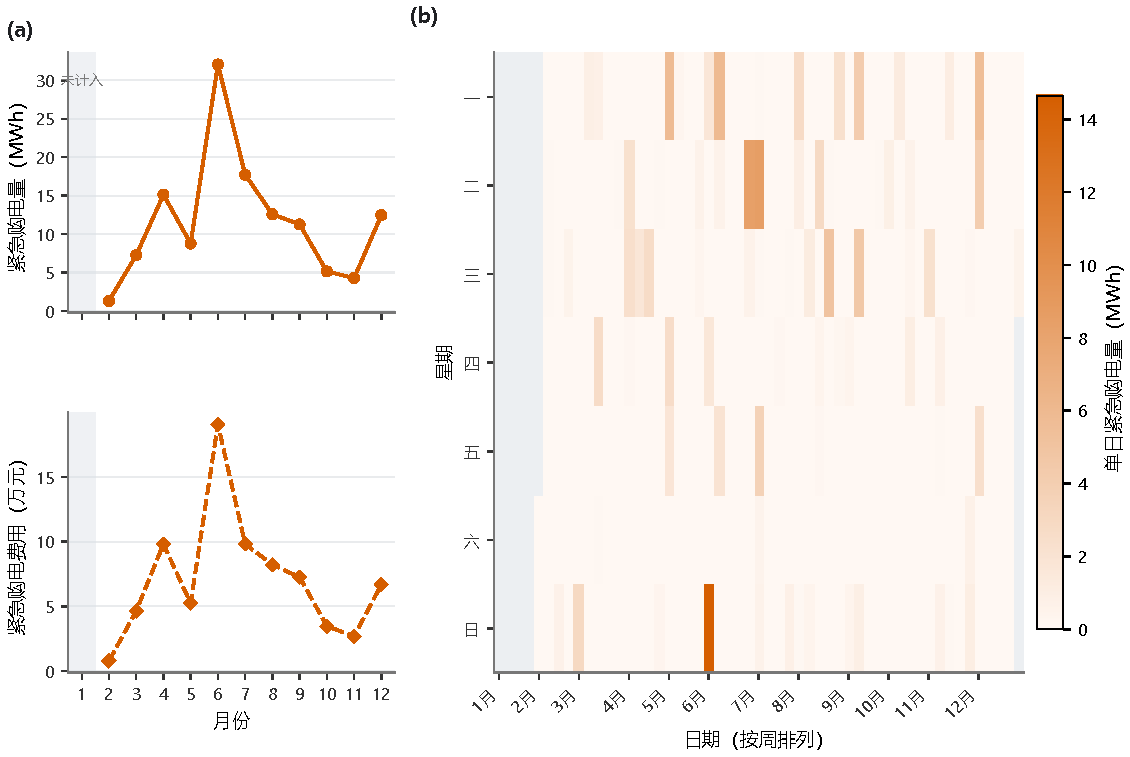
\includegraphics[width=.96\linewidth,height=8.5cm,keepaspectratio]{../new_figures_main/Q2_F3_annual_risk_profile.pdf}
\caption{统计期紧急购电的月度与逐日分布}
\figtabnote{1月为预热段，不纳入费用统计。}
\end{figure}
图6显示，紧急购电在6月较为集中，少数日期形成明显峰值。因此，日前平均费用之外还需关注应急需求的时间分布，以安排储能余量。
\par
\begin{figure}[H]\centering
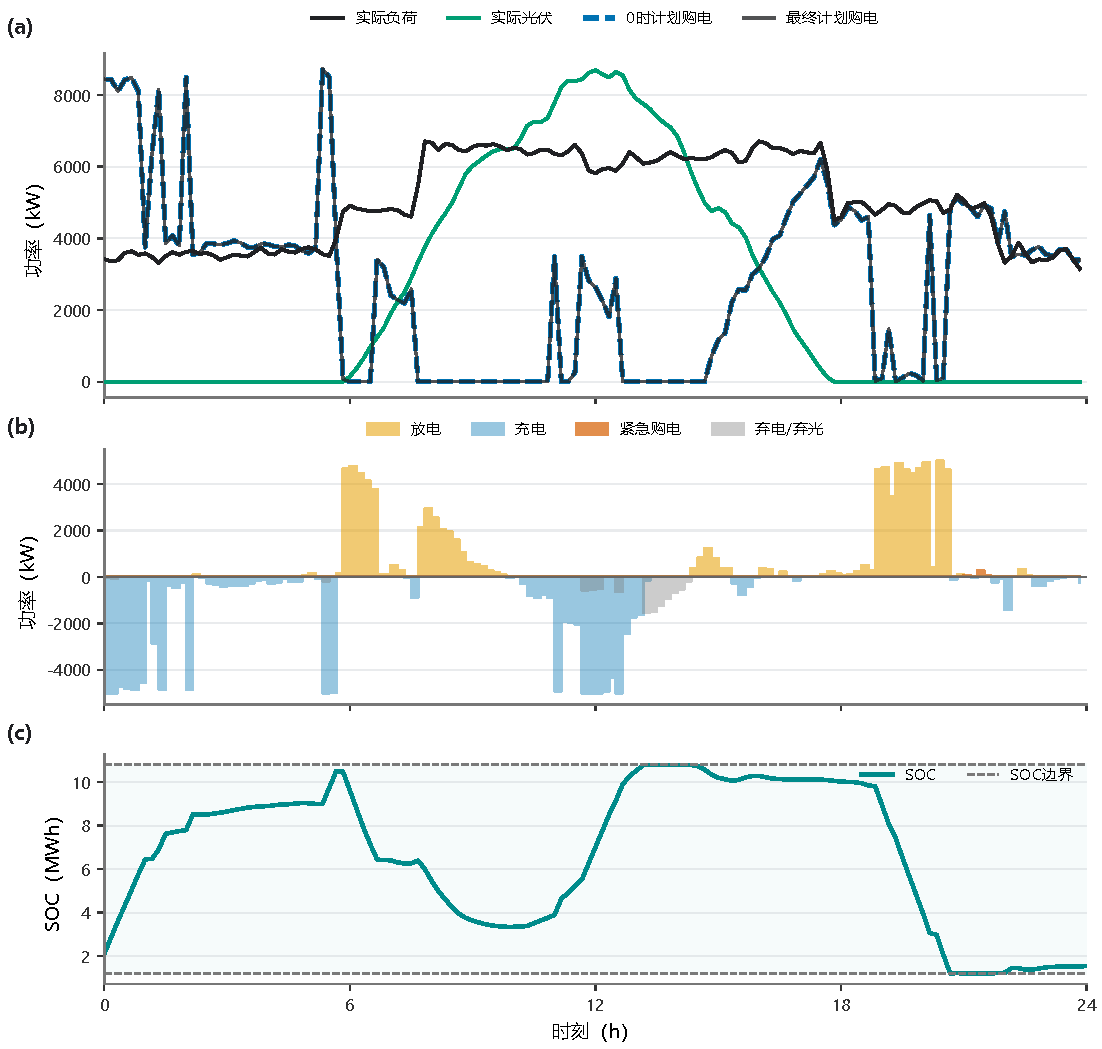
\includegraphics[width=.96\linewidth,height=11.0cm,keepaspectratio]{../new_figures_main/Q2_F1_typical_dispatch.pdf}
\caption{问题二典型日购电与储能运行}
\figtabnote{2025-09-23；购电曲线为计划购电，紧急购电另列。图中“弃电/弃光”表示全部余电。}
\end{figure}
图7进一步给出9月23日的运行过程。午间光伏富余使储能接近上边界，晚间持续放电后储能接近下边界，21时附近出现65.63 kWh紧急购电。日前计划在全天保持固定，预测偏差主要由储能吸收，超出可调能力的部分由紧急购电补足。
\par
以下按购电、储能、紧急购电三类结果汇总四个指定日期；同类结果按日期分组，保留题面表1—3的列次和字段。储能量按微网侧计量。
\par
\begin{table}[H]\centering
\fontsize{9.5}{12}\selectfont\setlength{\tabcolsep}{4pt}\renewcommand{\arraystretch}{1.12}
\begin{adjustbox}{max width=\linewidth}\begin{tabular}{lccccc}\toprule
\textbf{时间段} & \shortstack{\textbf{购电量}\\{\normalfont （kWh）}} & \textbf{时间段} & \shortstack{\textbf{购电量}\\{\normalfont （kWh）}} & \textbf{时间段} & \shortstack{\textbf{购电量}\\{\normalfont （kWh）}}\\
\midrule
\multicolumn{6}{l}{\textbf{2025-03-20}}\\[1pt]
10:00–10:10 & 0.00 & 12:00–12:10 & 625.40 & 14:00–14:10 & 0.00\\
16:00–16:10 & 455.28 & 18:00–18:10 & 671.19 & 20:00–20:10 & 0.00\\
全天购电量 & 66148.82 & 全天总费用/元 & 40940.02 & 单位 & kWh、元\\
\addlinespace[4pt]
\multicolumn{6}{l}{\textbf{2025-06-21}}\\[1pt]
10:00–10:10 & 0.00 & 12:00–12:10 & 0.00 & 14:00–14:10 & 0.00\\
16:00–16:10 & 179.07 & 18:00–18:10 & 193.13 & 20:00–20:10 & 0.00\\
全天购电量 & 33335.65 & 全天总费用/元 & 19637.89 & 单位 & kWh、元\\
\addlinespace[4pt]
\multicolumn{6}{l}{\textbf{2025-09-23}}\\[1pt]
10:00–10:10 & 0.00 & 12:00–12:10 & 439.89 & 14:00–14:10 & 0.00\\
16:00–16:10 & 527.13 & 18:00–18:10 & 752.85 & 20:00–20:10 & 3.63\\
全天购电量 & 66611.15 & 全天总费用/元 & 43062.88 & 单位 & kWh、元\\
\addlinespace[4pt]
\multicolumn{6}{l}{\textbf{2025-12-21}}\\[1pt]
10:00–10:10 & 0.00 & 12:00–12:10 & 856.43 & 14:00–14:10 & 0.00\\
16:00–16:10 & 813.89 & 18:00–18:10 & 678.35 & 20:00–20:10 & 0.00\\
全天购电量 & 94191.33 & 全天总费用/元 & 61188.39 & 单位 & kWh、元\\
\bottomrule\end{tabular}\end{adjustbox}
\caption{问题二指定日期购电量与全天费用}
\figtabnote{各日期沿用题面表1的列次；购电量单位为kWh，费用单位为元。}
\end{table}
\begin{table}[H]\centering
\fontsize{9.5}{12}\selectfont\setlength{\tabcolsep}{4pt}\renewcommand{\arraystretch}{1.12}
\begin{adjustbox}{max width=\linewidth}\begin{tabular}{lccccc}\toprule
\textbf{时间段} & \textbf{充电量} & \textbf{放电量} & \textbf{时间段} & \textbf{充电量} & \textbf{放电量}\\
\midrule
\multicolumn{6}{l}{\textbf{2025-03-20}}\\[1pt]
00:00–04:00 & 7146.43 & 164.49 & 04:00–08:00 & 2130.64 & 4704.60\\
08:00–12:00 & 5033.40 & 2777.38 & 12:00–16:00 & 4620.42 & 501.13\\
16:00–20:00 & 34.33 & 5509.90 & 20:00–24:00 & 681.65 & 2906.81\\
0:00储电量 & 2541.29 & — & 24:00储电量 & 1818.69 & —\\
\addlinespace[4pt]
\multicolumn{6}{l}{\textbf{2025-06-21}}\\[1pt]
00:00–04:00 & 425.71 & 415.84 & 04:00–08:00 & 1182.56 & 1843.75\\
08:00–12:00 & 10168.34 & 0.00 & 12:00–16:00 & 0.00 & 0.00\\
16:00–20:00 & 33.10 & 5057.02 & 20:00–24:00 & 751.22 & 2595.70\\
0:00储电量 & 2711.70 & — & 24:00储电量 & 3002.87 & —\\
\addlinespace[4pt]
\multicolumn{6}{l}{\textbf{2025-09-23}}\\[1pt]
00:00–04:00 & 7572.93 & 17.01 & 04:00–08:00 & 1976.79 & 4704.25\\
08:00–12:00 & 4078.03 & 1896.62 & 12:00–16:00 & 4448.31 & 660.67\\
16:00–20:00 & 24.02 & 5699.28 & 20:00–24:00 & 498.69 & 2583.15\\
0:00储电量 & 2107.46 & — & 24:00储电量 & 1556.39 & —\\
\addlinespace[4pt]
\multicolumn{6}{l}{\textbf{2025-12-21}}\\[1pt]
00:00–04:00 & 8110.27 & 183.59 & 04:00–08:00 & 2652.95 & 1604.01\\
08:00–12:00 & 5355.11 & 6619.39 & 12:00–16:00 & 7222.51 & 2433.99\\
16:00–20:00 & 56.39 & 5377.06 & 20:00–24:00 & 386.15 & 2962.32\\
0:00储电量 & 1823.00 & — & 24:00储电量 & 1916.51 & —\\
\bottomrule\end{tabular}\end{adjustbox}
\caption{问题二指定日期储能充放电及首末储电量（kWh）}
\figtabnote{各日期沿用题面表2的列次。}
\end{table}

\begin{table}[H]\centering
\fontsize{9.5}{12}\selectfont\setlength{\tabcolsep}{4pt}\renewcommand{\arraystretch}{1.12}
\begin{adjustbox}{max width=\linewidth}\begin{tabular}{lccccccc}\toprule
\multicolumn{2}{c}{\textbf{03-20}} & \multicolumn{2}{c}{\textbf{06-21}} & \multicolumn{2}{c}{\textbf{09-23}} & \multicolumn{2}{c}{\textbf{12-21}}\\
\cmidrule(lr){1-2} \cmidrule(lr){3-4} \cmidrule(lr){5-6} \cmidrule(lr){7-8}
\textbf{时段} & \shortstack{\textbf{购电量}\\{\normalfont （kWh）}} & \textbf{时段} & \shortstack{\textbf{购电量}\\{\normalfont （kWh）}} & \textbf{时段} & \shortstack{\textbf{购电量}\\{\normalfont （kWh）}} & \textbf{时段} & \shortstack{\textbf{购电量}\\{\normalfont （kWh）}}\\\midrule
无 & 0.00 & 无 & 0.00 & 21:00–21:10 & 11.80 & 无 & 0.00\\
— & — & — & — & 21:20–21:40 & 53.83 & — & —\\
合计 & 0.00 & 合计 & 0.00 & 合计 & 65.63 & 合计 & 0.00\\
\bottomrule\end{tabular}\end{adjustbox}
\caption{问题二四个典型日紧急购电（kWh）}
\end{table}
\section{6 问题三：预报组合与日内滚动调整}
\subsection{6.1 预报对齐、组合及当日修正}
附件3的整点预报先线性插值到10分钟右端点网格。0时发布时以0作为边界锚点；6、12、18时发布时，以该时刻之前最后一个已完成时段的光伏观测为边界锚点，再连接至发布后第一个整点预报。仅提取当日剩余时段，未将次日部分纳入跨午夜的优化。
\par
设$A_{i,t}^{\tau}$为附件3插值预报，$H_{i,t}$为历史均值预测。按最近30天同一发布时间、同一剩余时域的MAE选择组合权重：
\par
\begin{equation}
w_i^{\tau}\in\arg\min_{w\in\{0,0.1,\ldots,1\}}\frac{1}{|\mathcal H_i|(144-\tau)}\sum_{h\in\mathcal H_i}\sum_{t=\tau}^{143}\left|wA_{h,t}^{\tau}+(1-w)H_{h,t}-P^G_{h,t}\right|. \tag{12}
\end{equation}
由此得到$\widehat P_{i,t}^{G,\tau}=w_i^{\tau}A_{i,t}^{\tau}+(1-w_i^{\tau})H_{i,t}$。集合$\mathcal H_i$只含日期$i$以前的样本，权重不使用当前日剩余时段的真实光伏。
\par
日内负载修正利用当日已观测误差。设其均值为$b$、最近一个误差为$u$，对距更新时刻第$\ell$个时段的预测采用
\par
\begin{equation}
\widehat P_{t}^{L,\tau}=\left[\widehat P_t^{L,0}+b+0.65^{\ell}(u-b)\right]_+. \tag{13}
\end{equation}
光伏修正取更新前最近一个0时组合预测大于1 kW的时段$a$，以$\kappa=P^G_a/\widehat P_a^{G,0}$表示实际出力相对原预测的比例；不存在该时段时令$\kappa=1$。按距离衰减该比例偏差：
\par
\begin{equation}
\widetilde P_t^{G,\tau}=\left[\widehat P_t^{G,\tau}\{1+(\kappa-1)0.94^{\ell}\}\right]_+. \tag{14}
\end{equation}
式（14）按实际光伏相对于0时组合预测的比例修正剩余时段，随后基于更新预测形成相应的历史残差场景。
\par
\subsection{6.2 原计划、调整变量与结算模型}
将0时计划记为$g_t^0$。对每条场景设置减购量$r_t^k$和增购量$x_t^k$，6时以前二者固定为0，6时及以后允许追索，且$0\le r_t^k\le g_t^0$。在0时提前考虑未来可能调整的代价：
\par
\begin{equation}
\begin{aligned}
\min\;&\sum_t\pi_tg_t^0+\frac1K\sum_k\Big[\sum_t\pi_t(-0.5r_t^k+1.5x_t^k+5e_t^k)\\
&\hspace{32mm}+\epsilon\sum_t(c_t^k+d_t^k)-vS_{144}^k\Big].
\end{aligned} \tag{15}
\end{equation}
各场景电量平衡中的计划电量相应替换为$g_t^0-r_t^k+x_t^k$。式（15）的场景减购、增购代表提前评估的补救机会，实际执行的调整仍须在信息发布后重新求解。
\par
在$\tau=36,72,108$，以当前实际储电量为初值，更新负载、光伏及残差场景，对剩余时段使用共同调整决策：
\par
\begin{equation}
g_t^{\tau}=g_t^0-r_t^{\tau}+x_t^{\tau},\qquad0\le r_t^{\tau}\le g_t^0,\quad x_t^{\tau}\ge0,\quad t\ge\tau. \tag{16}
\end{equation}
滚动目标为剩余调整费用与平均场景应急、吞吐和终端代价之和，约束与问题二相同。0时承诺费用为常数，式（16）的调整量始终以0时原计划为基准。
\par
最终计划按实际适用时段拼接：0—6时用$g^0$，6—12时用$g^{36}$，12—18时用$g^{72}$，18—24时用$g^{108}$。记拼接结果为$g^{\mathrm{fin}}$，则总费用为
\par
\begin{equation}
\begin{aligned}
C_3&=C_{\mathrm{plan}}+C_{\mathrm{adj}}+C_{\mathrm{em}},\\
C_{\mathrm{plan}}&=\sum_{i,t}\pi_tg_{i,t}^0,\\
C_{\mathrm{adj}}&=\sum_{i,t}\pi_t\left[-0.5(g_{i,t}^0-g_{i,t}^{\mathrm{fin}})_++1.5(g_{i,t}^{\mathrm{fin}}-g_{i,t}^0)_+\right],\\
C_{\mathrm{em}}&=5\sum_{i,t}\pi_te_{i,t}.
\end{aligned} \tag{17}
\end{equation}
例如原计划100 kWh、最终80 kWh，按100倍单价计入计划费，再减去10倍单价的调整退款，等价于80 kWh购电费与20 kWh减购量的50\%违约费。
\par
\begin{figure}[H]\centering
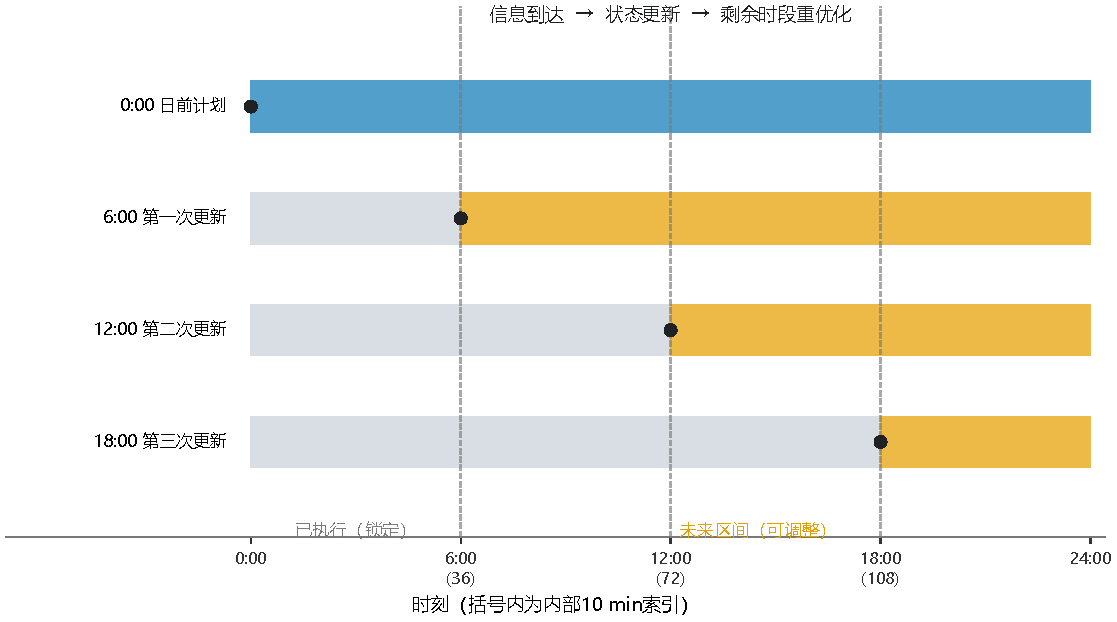
\includegraphics[width=.96\linewidth,height=6.3cm,keepaspectratio]{../new_figures_main/Q3_F1_rolling_timeline.pdf}
\caption{问题三信息更新与剩余时段调整}
\figtabnote{已执行时段锁定，每次更新以当前实测储电量为起点。}
\end{figure}
\subsection{6.3 预报效果与运行费用}
\begin{figure}[H]\centering
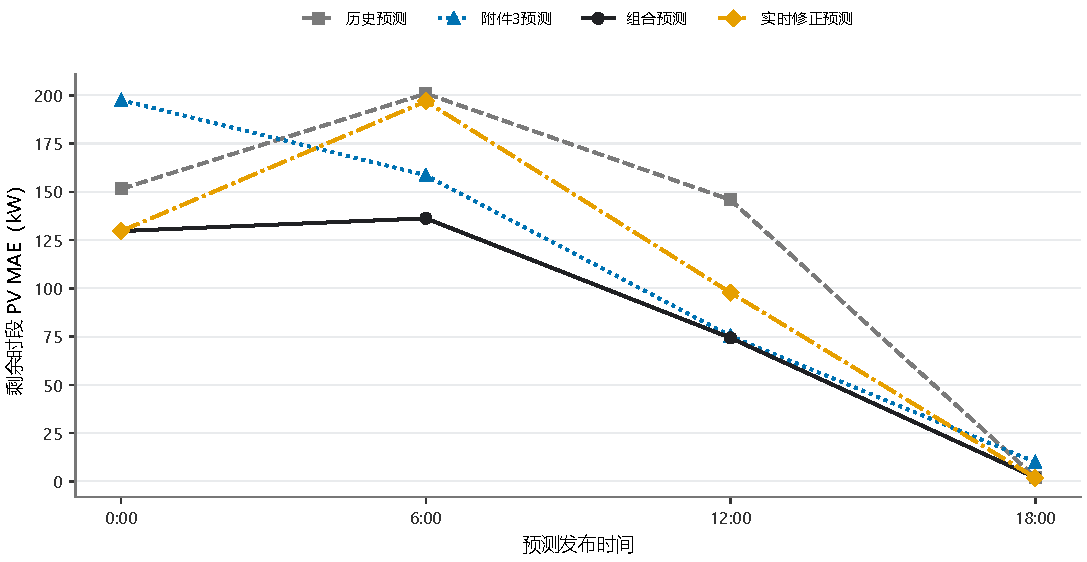
\includegraphics[width=.96\linewidth,height=6.7cm,keepaspectratio]{../new_figures_main/Q3_F2_forecast_improvement.pdf}
\caption{各发布时间的光伏预测误差}
\figtabnote{MAE按各次发布后的当日剩余时段计算。}
\end{figure}
图9中，组合预测在四个发布时间的MAE均低于直接使用附件3。比例修正却使6时MAE从136.26增至196.90 kW、12时从74.32增至97.79 kW，说明近期出力比例延伸到未来时可能放大天气偏差。18时剩余时段以低出力为主，四条误差曲线随之接近；同一发布时间下的比较更能反映方法差别。
\par

统计期汇总显示，主方案较问题二节约43.50万元，其中计划费降低51.72万元、紧急购电费降低67.16万元，抵消了新增的75.37万元调整费。紧急购电量由127912.33降至21152.53 kWh，减少83.46\%。节约来自计划、预报与执行方式共同改变后的综合效果。
\par
统计期节约并非每天都发生：四个指定日期的主方案费用均高于问题二，具体见第6.5节的典型日结果。日内调整的付费成本与应急支出需要在完整统计期内共同评价。
\par
\subsection{6.4 额外发布时间的必要性}
\begin{figure}[H]\centering
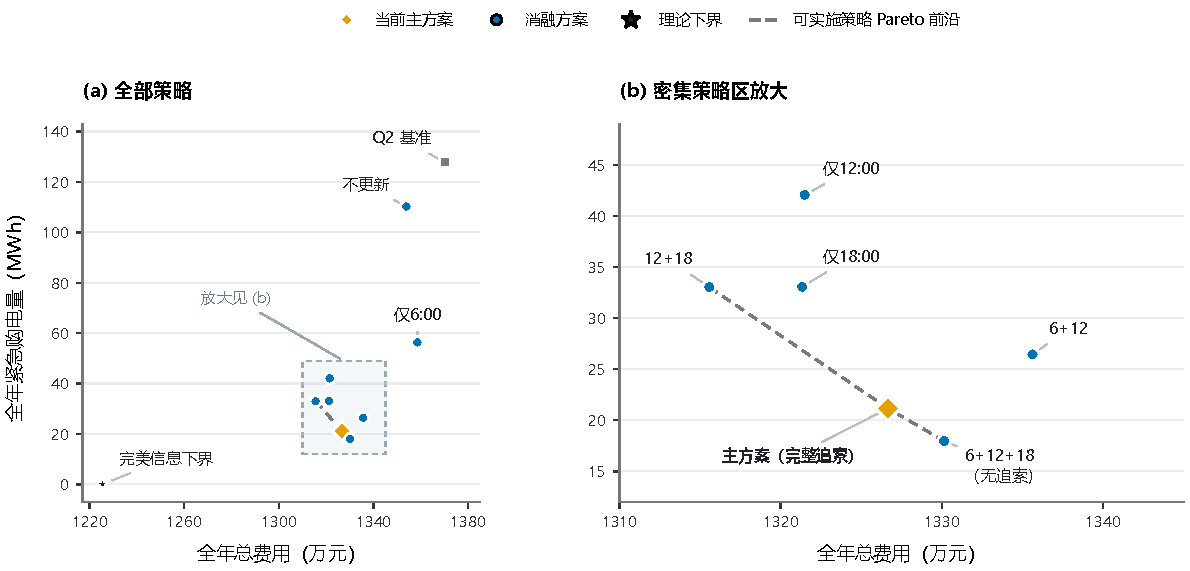
\includegraphics[width=.96\linewidth,height=7.6cm,keepaspectratio]{../new_figures_main/Q3_F3_strategy_pareto.pdf}
\caption{滚动方案的费用与紧急购电量比较}
\figtabnote{图中“理论下界”为原图对完美信息参照的标记；该参照采用逐日优化与终端价值，并非统计期费用的严格下界。}
\end{figure}
图10给出各方案的费用与紧急购电量。仅6时更新的费用高于不更新；仅12时或仅18时更新均降低费用，12、18时组合的费用最低，为1315.58万元。可实施方案的非支配前沿由12+18时、完整追索主方案及6+12+18时无追索方案构成，分别体现费用与应急需求之间的取舍。
\par
主方案比12、18时方案多支出11.08万元，紧急购电量减少11877.23 kWh。固定6、12、18时更新后，加入日前追索使费用由1330.14降至1326.66万元，紧急购电量却从17970.87增至21152.53 kWh。因此，选择12、18时更新偏重费用目标，完整追索主方案则在较低费用与较小应急量之间折中。
\par
上述前沿和最低费用均对应已比较的方案集合。完美信息点作为参照单独列示，不参与可实施方案前沿的计算。
\par
\subsection{6.5 典型日计划演化与费用比较}
\begin{figure}[H]\centering
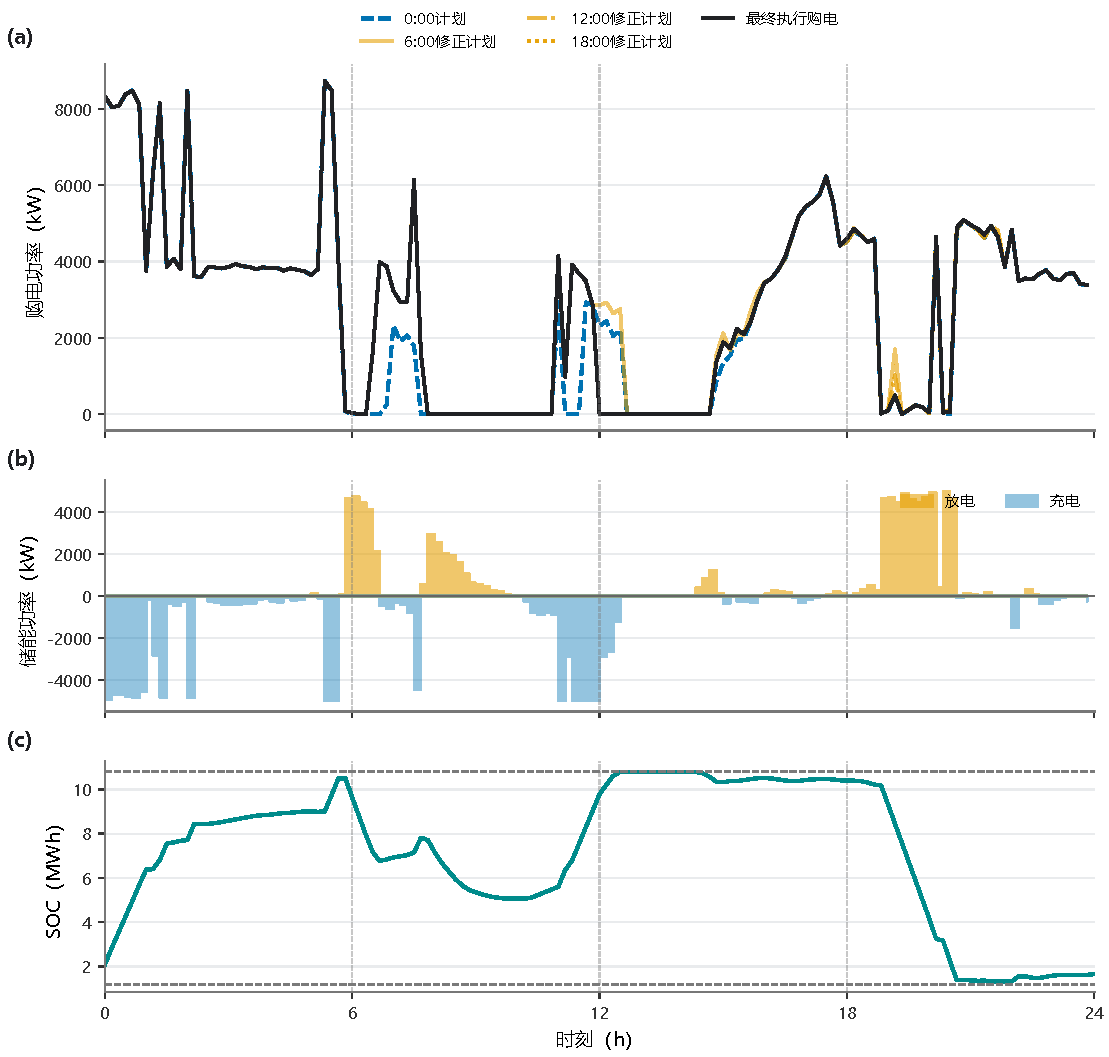
\includegraphics[width=.96\linewidth,height=11.0cm,keepaspectratio]{../new_figures_main/Q3_F4_plan_evolution.pdf}
\caption{问题三典型日购电计划的滚动演化}
\figtabnote{2025-09-23；竖虚线为6、12、18时的信息发布时刻。}
\end{figure}
图11以9月23日为例：各次修正只延伸到发布后的时段，实线最终计划由最近一次可用方案拼接而成。午间与晚间购电量随新信息调整，储能在白天补充电量、晚间释放，晚间紧急购电由问题二的65.63 kWh降至0。
\par
以下按日期分组汇总题面要求的三类结果：购电量以“原计划/最终计划”列示，储能表列最终运行结果，紧急购电表按四个日期并列。
\par
\begin{table}[H]\centering
\fontsize{9.5}{12}\selectfont\setlength{\tabcolsep}{4pt}\renewcommand{\arraystretch}{1.12}
\begin{adjustbox}{max width=\linewidth}\begin{tabular}{lccccc}\toprule
\textbf{时间段} & \shortstack{\textbf{购电量}\\{\normalfont （kWh）}} & \textbf{时间段} & \shortstack{\textbf{购电量}\\{\normalfont （kWh）}} & \textbf{时间段} & \shortstack{\textbf{购电量}\\{\normalfont （kWh）}}\\
\midrule
\multicolumn{6}{l}{\textbf{2025-03-20}}\\[1pt]
10:00–10:10 & 0.00 / 0.00 & 12:00–12:10 & 538.09 / 618.49 & 14:00–14:10 & 0.00 / 0.00\\
16:00–16:10 & 538.26 / 538.26 & 18:00–18:10 & 671.19 / 679.70 & 20:00–20:10 & 0.00 / 0.00\\
全天购电量 & 65024.60 / 65917.49 & 全天总费用/元 & 44142.02 & 单位 & kWh、元\\
\addlinespace[4pt]
\multicolumn{6}{l}{\textbf{2025-06-21}}\\[1pt]
10:00–10:10 & 0.00 / 0.00 & 12:00–12:10 & 0.00 / 0.00 & 14:00–14:10 & 0.00 / 0.00\\
16:00–16:10 & 128.77 / 128.77 & 18:00–18:10 & 0.00 / 0.00 & 20:00–20:10 & 0.00 / 0.00\\
全天购电量 & 32788.93 / 33321.63 & 全天总费用/元 & 19727.57 & 单位 & kWh、元\\
\addlinespace[4pt]
\multicolumn{6}{l}{\textbf{2025-09-23}}\\[1pt]
10:00–10:10 & 0.00 / 0.00 & 12:00–12:10 & 386.56 / 0.00 & 14:00–14:10 & 0.00 / 0.00\\
16:00–16:10 & 573.36 / 573.36 & 18:00–18:10 & 752.85 / 765.47 & 20:00–20:10 & 3.63 / 7.30\\
全天购电量 & 64801.74 / 68391.05 & 全天总费用/元 & 46234.62 & 单位 & kWh、元\\
\addlinespace[4pt]
\multicolumn{6}{l}{\textbf{2025-12-21}}\\[1pt]
10:00–10:10 & 0.00 / 0.00 & 12:00–12:10 & 894.78 / 894.78 & 14:00–14:10 & 0.00 / 0.00\\
16:00–16:10 & 823.30 / 847.49 & 18:00–18:10 & 666.26 / 446.98 & 20:00–20:10 & 0.00 / 0.00\\
全天购电量 & 93530.09 / 94363.30 & 全天总费用/元 & 61692.49 & 单位 & kWh、元\\
\bottomrule\end{tabular}\end{adjustbox}
\caption{问题三指定日期购电量与全天费用}
\figtabnote{购电量按“原计划/最终计划”列示，单位为kWh；费用单位为元。}
\end{table}
\begin{table}[H]\centering
\fontsize{9.5}{12}\selectfont\setlength{\tabcolsep}{4pt}\renewcommand{\arraystretch}{1.12}
\begin{adjustbox}{max width=\linewidth}\begin{tabular}{lccccc}\toprule
\textbf{时间段} & \textbf{充电量} & \textbf{放电量} & \textbf{时间段} & \textbf{充电量} & \textbf{放电量}\\
\midrule
\multicolumn{6}{l}{\textbf{2025-03-20}}\\[1pt]
00:00–04:00 & 7394.59 & 14.97 & 04:00–08:00 & 1829.31 & 5691.28\\
08:00–12:00 & 2935.78 & 2506.79 & 12:00–16:00 & 7072.08 & 255.20\\
16:00–20:00 & 153.57 & 5259.70 & 20:00–24:00 & 681.04 & 2717.52\\
0:00储电量 & 2024.09 & — & 24:00储电量 & 1811.09 & —\\
\addlinespace[4pt]
\multicolumn{6}{l}{\textbf{2025-06-21}}\\[1pt]
00:00–04:00 & 198.67 & 306.84 & 04:00–08:00 & 1389.78 & 1440.01\\
08:00–12:00 & 9670.60 & 0.00 & 12:00–16:00 & 0.00 & 0.00\\
16:00–20:00 & 41.50 & 5273.24 & 20:00–24:00 & 686.38 & 2623.75\\
0:00储电量 & 2607.81 & — & 24:00储电量 & 2680.65 & —\\
\addlinespace[4pt]
\multicolumn{6}{l}{\textbf{2025-09-23}}\\[1pt]
00:00–04:00 & 7513.62 & 5.55 & 04:00–08:00 & 3016.80 & 3965.15\\
08:00–12:00 & 5253.03 & 1896.62 & 12:00–16:00 & 1333.90 & 425.56\\
16:00–20:00 & 107.98 & 5807.95 & 20:00–24:00 & 479.75 & 2638.16\\
0:00储电量 & 2100.88 & — & 24:00储电量 & 1658.82 & —\\
\addlinespace[4pt]
\multicolumn{6}{l}{\textbf{2025-12-21}}\\[1pt]
00:00–04:00 & 8083.92 & 35.88 & 04:00–08:00 & 2938.42 & 1750.20\\
08:00–12:00 & 5069.31 & 7130.47 & 12:00–16:00 & 7958.21 & 2251.40\\
16:00–20:00 & 0.00 & 5621.05 & 20:00–24:00 & 413.06 & 2939.14\\
0:00储电量 & 1563.96 & — & 24:00储电量 & 1660.43 & —\\
\bottomrule\end{tabular}\end{adjustbox}
\caption{问题三指定日期储能充放电及首末储电量（kWh）}
\figtabnote{表中为最终实际运行结果。}
\end{table}

\begin{table}[H]\centering
\fontsize{9.5}{12}\selectfont\setlength{\tabcolsep}{4pt}\renewcommand{\arraystretch}{1.12}
\begin{adjustbox}{max width=\linewidth}\begin{tabular}{lccccccc}\toprule
\multicolumn{2}{c}{\textbf{03-20}} & \multicolumn{2}{c}{\textbf{06-21}} & \multicolumn{2}{c}{\textbf{09-23}} & \multicolumn{2}{c}{\textbf{12-21}}\\
\cmidrule(lr){1-2} \cmidrule(lr){3-4} \cmidrule(lr){5-6} \cmidrule(lr){7-8}
\textbf{时段} & \shortstack{\textbf{购电量}\\{\normalfont （kWh）}} & \textbf{时段} & \shortstack{\textbf{购电量}\\{\normalfont （kWh）}} & \textbf{时段} & \shortstack{\textbf{购电量}\\{\normalfont （kWh）}} & \textbf{时段} & \shortstack{\textbf{购电量}\\{\normalfont （kWh）}}\\\midrule
09:10–10:00 & 270.59 & 无 & 0.00 & 无 & 0.00 & 无 & 0.00\\
合计 & 270.59 & 合计 & 0.00 & 合计 & 0.00 & 合计 & 0.00\\
\bottomrule\end{tabular}\end{adjustbox}
\caption{问题三四个典型日紧急购电（kWh）}
\end{table}
典型日总费用与紧急购电量变化并不一致：9月23日虽消除了紧急购电，总费用仍增加；3月20日则发生270.59 kWh紧急购电。滚动策略的统计期节约由全年各日的费用变化共同形成。
\par
\section{7 问题四：波动电价下的因果购电策略}
\subsection{7.1 价格信息与决策规则}
价格波动同时改变储能转移电量的收益、紧急购电和调整成本。0时电价预测取最近三个同类型日均值$\widehat\pi_{i,t}^{0}$；历史不足时使用已有样本，最初以附件1价格启动。日内利用已观测价格的累计水平修正剩余预测：
\par
\begin{equation}
a_i^{\tau}=\frac{\sum_{t<\tau}\pi_{i,t}}{\sum_{t<\tau}\widehat\pi_{i,t}^{0}},\qquad \widehat\pi_{i,t}^{\tau}=a_i^{\tau}\widehat\pi_{i,t}^{0},\quad t\ge\tau. \tag{18}
\end{equation}
该比例改变剩余曲线的整体水平，保留其峰谷位置。问题四之二将式（8）的价格替换为0时预测价格；问题四之三还在6、12、18时更新滚动目标。两者均按附件4实际交易价格结算式（11）、式（17）的费用。
\par
图12中，价格MAE约为0.036—0.040元/kWh，6时更新后略升、18时最低。不同发布时间的剩余样本与价格突变不同，比例修正只能调整整体水平，因此误差变化并非单调。
\par
\begin{figure}[H]\centering
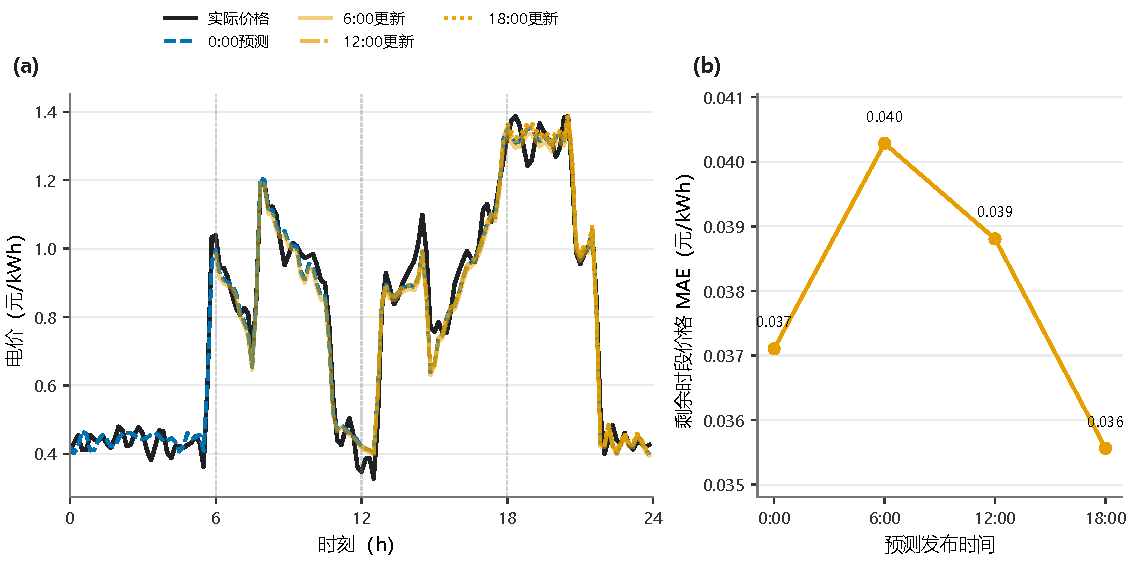
\includegraphics[width=.96\linewidth,height=7.0cm,keepaspectratio]{../new_figures_main/Q4_F2_price_forecast_update.pdf}
\caption{典型日电价更新与统计期预测误差}
\figtabnote{各次预测仅覆盖发布后的未来区间。}
\end{figure}
\subsection{7.2 统计期费用与信息价值}

统计期因果日前与滚动方案费用分别为1440.18、1395.35万元，滚动方案节约44.83万元，即3.11\%；紧急购电量从126055.49降至22900.97 kWh，减少81.83\%。
\par
\begin{figure}[H]\centering
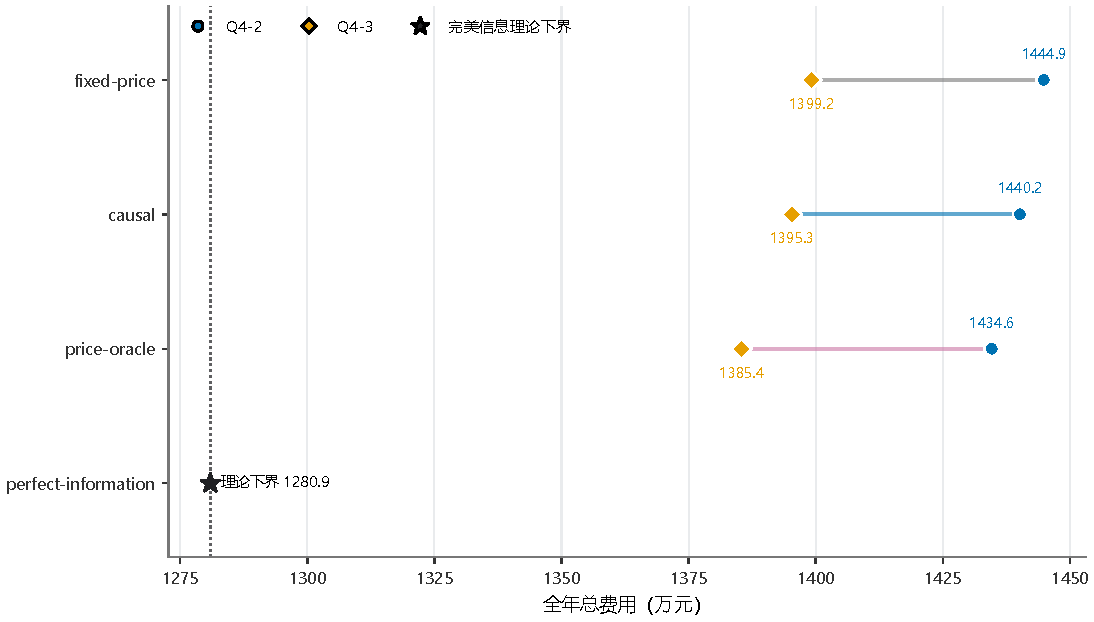
\includegraphics[width=.96\linewidth,height=7.2cm,keepaspectratio]{../new_figures_main/Q4_F1_information_value.pdf}
\caption{不同价格信息下的日前与滚动费用}
\figtabnote{各点统一按实际电价结算；price-oracle为预知电价对照，“理论下界”为与图10同义的完美信息参照。}
\end{figure}
图13区分价格信息条件：fixed-price使用附件1固定价格决策，causal使用当时可得的价格预测，price-oracle预知当天实际价格而仍预测负载与光伏；三者统一按附件4实际价格结算。相对固定价格决策，因果预测使日前、滚动方案分别节约0.33\%、0.27\%；进一步预知电价后，再分别节约0.39\%、0.71\%。本组对照中，滚动调整的费用差大于价格预测相对固定价格的费用差。
\par
完美信息参照同时已知负载、光伏与电价，其费用为1280.93万元，用于衡量当前策略与充分信息条件下参考表现的差距。
\par
\subsection{7.3 价格、储能与购电的日内配合}

\begin{figure}[H]\centering
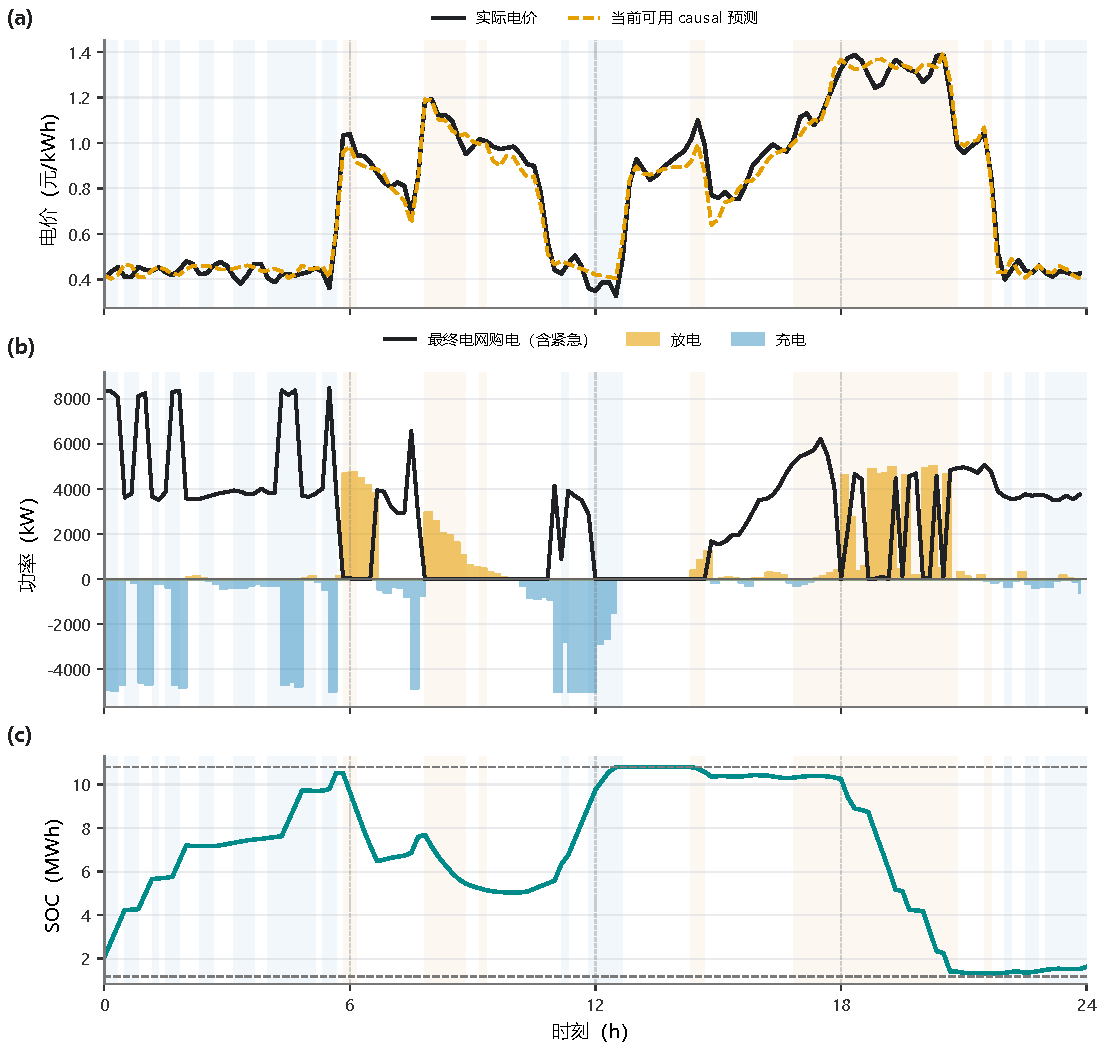
\includegraphics[width=.96\linewidth,height=11.0cm,keepaspectratio]{../new_figures_main/Q4_F3_price_dispatch_coupling.pdf}
\caption{波动电价下的储能与购电配合}
\figtabnote{2025-09-23；最终电网购电含紧急购电。背景按实际价格P25/P75划分低/高价区间，仅作事后解释。}
\end{figure}
问题四之二为日前方案，问题四之三为滚动方案；四个指定日期的滚动费用均高于日前方案。图14选取9月23日，该日紧急购电由67.16降至7.77 kWh，总费用却增加3297.27元；低价充电、高价放电减少了晚间缺口，调整成本仍需一并计入费用。统计期的净节约来自其他日期的改善。
\par
沿用题面指定日期和时段，以下将波动电价下两种方案并列，给出购电、储能及紧急购电结果。
\par
\begin{table}[H]\centering
\fontsize{9.5}{12}\selectfont\setlength{\tabcolsep}{4pt}\renewcommand{\arraystretch}{1.12}
\begin{adjustbox}{max width=\linewidth}\begin{tabular}{lccccc}\toprule
\textbf{时间段} & \textbf{方案} & \textbf{03-20} & \textbf{06-21} & \textbf{09-23} & \textbf{12-21}\\
\midrule
10:00–10:10 & 日前 & 0.00 & 0.00 & 0.00 & 0.00\\
10:00–10:10 & 滚动 & 0.00 & 0.00 & 0.00 & 0.00\\
\addlinespace[2pt]
12:00–12:10 & 日前 & 625.40 & 0.00 & 439.89 & 856.43\\
12:00–12:10 & 滚动 & 618.49 & 0.00 & 0.00 & 865.61\\
\addlinespace[2pt]
14:00–14:10 & 日前 & 0.00 & 0.00 & 0.00 & 0.00\\
14:00–14:10 & 滚动 & 0.00 & 0.00 & 0.00 & 0.00\\
\addlinespace[2pt]
16:00–16:10 & 日前 & 465.12 & 137.16 & 527.13 & 813.89\\
16:00–16:10 & 滚动 & 538.26 & 128.77 & 586.22 & 847.49\\
\addlinespace[2pt]
18:00–18:10 & 日前 & 671.07 & 13.22 & 0.00 & 729.95\\
18:00–18:10 & 滚动 & 671.07 & 0.00 & 0.00 & 439.00\\
\addlinespace[2pt]
20:00–20:10 & 日前 & 692.15 & 0.00 & 3.63 & 0.00\\
20:00–20:10 & 滚动 & 694.56 & 0.00 & 7.30 & 0.00\\
全天原计划购电量 & 日前 & 66219.79 & 33748.13 & 66834.10 & 84525.79\\
全天原计划购电量 & 滚动 & 64782.09 & 33488.12 & 64822.50 & 83961.70\\
\addlinespace[2pt]
全天最终购电量 & 日前 & 66219.79 & 33748.13 & 66834.10 & 84525.79\\
全天最终购电量 & 滚动 & 65664.91 & 34062.20 & 68353.96 & 84524.30\\
\addlinespace[2pt]
全天总费用/元 & 日前 & 42083.51 & 17278.64 & 44970.74 & 67455.10\\
全天总费用/元 & 滚动 & 45045.32 & 17432.29 & 48268.01 & 68102.79\\
\addlinespace[2pt]
\bottomrule\end{tabular}\end{adjustbox}
\caption{问题四指定时段购电量、全天购电量与总费用}
\figtabnote{各时段列最终购电量，单位为kWh；“日前/滚动”分别对应问题四之二、之三。}
\end{table}
\begin{table}[H]\centering
\fontsize{9.5}{12}\selectfont\setlength{\tabcolsep}{4pt}\renewcommand{\arraystretch}{1.12}
\begin{adjustbox}{max width=\linewidth}\begin{tabular}{lccccc}\toprule
\textbf{时间段} & \textbf{方案} & \textbf{03-20} & \textbf{06-21} & \textbf{09-23} & \textbf{12-21}\\\midrule
00:00–04:00 & 日前 & 6653.96 / 247.10 & 166.36 / 1006.41 & 6284.54 / 30.55 & 507.30 / 229.56\\
00:00–04:00 & 滚动 & 6642.55 / 64.13 & 216.13 / 1014.16 & 6123.17 / 27.37 & 686.52 / 225.83\\
\addlinespace[2pt]
04:00–08:00 & 日前 & 2694.12 / 5133.41 & 1658.56 / 1755.02 & 4136.82 / 5339.30 & 316.74 / 971.38\\
04:00–08:00 & 滚动 & 1920.71 / 5713.74 & 2113.23 / 1371.89 & 4697.30 / 4162.08 & 326.01 / 1215.06\\
\addlinespace[2pt]
08:00–12:00 & 日前 & 5100.87 / 2777.38 & 10154.81 / 0.00 & 3930.46 / 1896.62 & 5011.80 / 6682.35\\
08:00–12:00 & 滚动 & 2904.15 / 2525.53 & 9663.15 / 0.00 & 5237.99 / 1896.62 & 5016.64 / 7135.31\\
\addlinespace[2pt]
12:00–16:00 & 日前 & 4594.71 / 527.79 & 0.00 / 0.00 & 4607.12 / 645.85 & 7318.90 / 2434.25\\
12:00–16:00 & 滚动 & 7112.77 / 254.72 & 0.00 / 0.00 & 1263.59 / 421.50 & 8000.11 / 2251.40\\
\addlinespace[2pt]
16:00–20:00 & 日前 & 27.96 / 6612.76 & 59.27 / 5157.66 & 24.02 / 5705.14 & 88.40 / 5307.03\\
16:00–20:00 & 滚动 & 115.61 / 6197.15 & 46.92 / 5317.66 & 110.62 / 5701.61 & 0.00 / 5621.03\\
\addlinespace[2pt]
20:00–24:00 & 日前 & 1201.75 / 1766.24 & 1410.14 / 2621.53 & 493.21 / 2595.02 & 452.32 / 3006.59\\
20:00–24:00 & 滚动 & 1176.75 / 1737.37 & 1340.32 / 2659.30 & 450.37 / 2668.98 & 445.38 / 2961.01\\
\addlinespace[2pt]
日初 / 日末 & 日前 & 3008.05 / 2293.32 & 3086.50 / 3478.93 & 2063.73 / 1578.42 & 10408.89 / 2033.49\\
日初 / 日末 & 滚动 & 2719.07 / 2279.19 & 2657.91 / 3185.22 & 2061.60 / 1625.04 & 10204.32 / 1665.23\\
\bottomrule\end{tabular}\end{adjustbox}
\caption{波动电价下典型日储能量（kWh）}
\figtabnote{单元格依次列出充电量与放电量；末两行为日初和日末储电量。}
\end{table}
\begin{table}[H]\centering
\fontsize{9.5}{12}\selectfont\setlength{\tabcolsep}{4pt}\renewcommand{\arraystretch}{1.12}
\begin{adjustbox}{max width=\linewidth}\begin{tabular}{lccccccc}\toprule
\multicolumn{2}{c}{\textbf{03-20}} & \multicolumn{2}{c}{\textbf{06-21}} & \multicolumn{2}{c}{\textbf{09-23}} & \multicolumn{2}{c}{\textbf{12-21}}\\
\cmidrule(lr){1-2} \cmidrule(lr){3-4} \cmidrule(lr){5-6} \cmidrule(lr){7-8}
\textbf{时段} & \shortstack{\textbf{购电量}\\{\normalfont （kWh）}} & \textbf{时段} & \shortstack{\textbf{购电量}\\{\normalfont （kWh）}} & \textbf{时段} & \shortstack{\textbf{购电量}\\{\normalfont （kWh）}} & \textbf{时段} & \shortstack{\textbf{购电量}\\{\normalfont （kWh）}}\\
\midrule
\multicolumn{8}{l}{\textbf{日前方案（问题四之二）}}\\[1pt]
无 & 0.00 & 无 & 0.00 & 20:10–20:20 & 10.00 & 无 & 0.00\\
— & — & — & — & 21:00–21:10 & 5.66 & — & —\\
— & — & — & — & 21:20–21:40 & 51.50 & — & —\\
合计 & 0.00 & 合计 & 0.00 & 合计 & 67.16 & 合计 & 0.00\\
\addlinespace[4pt]
\multicolumn{8}{l}{\textbf{滚动方案（问题四之三）}}\\[1pt]
09:10–10:00 & 251.85 & 无 & 0.00 & 20:10–20:20 & 7.77 & 无 & 0.00\\
合计 & 251.85 & 合计 & 0.00 & 合计 & 7.77 & 合计 & 0.00\\
\bottomrule\end{tabular}\end{adjustbox}
\caption{问题四两种方案在指定日期的紧急购电（kWh）}
\end{table}

\subsection{7.4 保持日均价格的波动灵敏度}
直接放大价格会同时改变平均购电成本和波动强度，难以区分二者作用。因此以每日电价的对数偏离构造压力情形，并保持每日算术平均价不变：
\par
\begin{equation}
u_{i,t}^{(\lambda)}=\exp\{\lambda(\log\pi_{i,t}-\overline{\log\pi_i})\},\qquad
\pi_{i,t}^{(\lambda)}=\overline\pi_i\frac{u_{i,t}^{(\lambda)}}{\overline{u_i^{(\lambda)}}}. \tag{19}
\end{equation}
其中横线表示日内144个时段的算术平均，$\lambda$取0.50、0.75、1.00、1.25、1.50。已有五组试验均按变换后的历史价格预测并调度，$\lambda=1$对应原始电价。
\par
图15中，滚动方案节约额由18.04增至64.34万元，节约率由1.17\%增至4.76\%，同期日内价格变异系数均值由0.219增至0.615。日均价格保持不变时，更大的峰谷差提高了调整购电时点与储能转移电量的价值。
\par
\begin{figure}[H]\centering
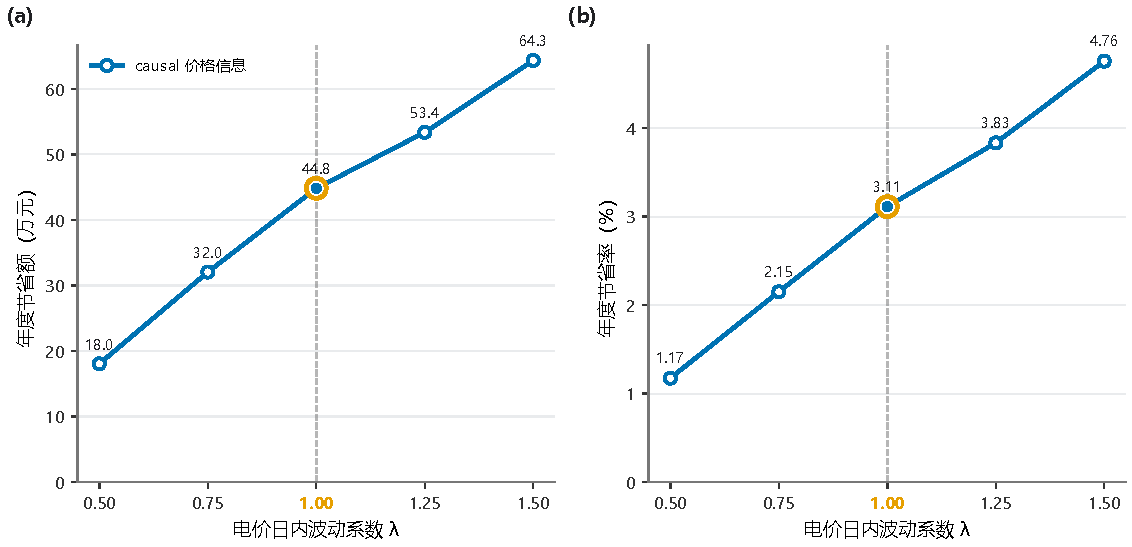
\includegraphics[width=.96\linewidth,height=7.0cm,keepaspectratio]{../new_figures_main/Q4_F4_rolling_gain_sensitivity.pdf}
\caption{电价波动强度与滚动调整节约}
\figtabnote{仅比较因果价格条件下的五组既有情形，日均价格保持不变。}
\end{figure}
\section{8 模型检验}
预测误差按决策时已生成的预测与随后出现的实际观测计算。设对应评价样本数为$M$，则
\par
\begin{equation}
\mathrm{MAE}=\frac1M\sum_{j=1}^M|\widehat P_j-P_j|,\qquad
\mathrm{RMSE}=\sqrt{\frac1M\sum_{j=1}^M(\widehat P_j-P_j)^2}. \tag{20}
\end{equation}
光伏夜间大量为零，采用MAE和RMSE避免百分比误差的分母问题；各次发布均在当日剩余时段评价。
\par

已有数值检查中，电量平衡最大残差为$4.55\times10^{-13}$ kWh，SOC递推最大残差为$9.09\times10^{-13}$ kWh；储电量处于1200—10800 kWh内，跨日状态连续，统计期费用与工作簿一致。表格数据均在未舍入结果上汇总后保留相应精度。
\par
问题一的线性规划解没有同时充放电；问题二至四的实际执行规则按供需缺口的符号选择充电或放电，实际轨迹的同时充放电时段数为0。
\par
\section{9 模型评价与应用建议}
\subsection{9.1 模型优点}
模型以日前承诺、付费调整和实时供电三个环节组织决策，将五倍紧急购电成本与储能容量、功率约束纳入同一费用框架。配对历史残差保留负载与光伏的共同波动，跨日SOC连续传递，使费用评价包含前一日储能决策的影响。
\par
预报更新既用误差曲线评价，也用费用与紧急购电量检验；价格对照统一实际结算环境，便于区分购电时点调整与价格信息的作用。
\par
\subsection{9.2 模型不足与可行改进}
问题一与后续各问的功率上限计量侧不同，设备应用时需按铭牌明确对应边界。十日残差与固定裕度对极端偏差的覆盖有限，两阶段补救也比真实逐时信息更充分；增加多年度样本可检验场景与裕度的适用性。
\par
光伏比例修正在6时和12时放大平均误差，可考虑按历史表现设置启用条件；电价比例修正仅调整整体水平，峰谷移动仍是其主要误差来源。
\par
模型以购电费用为目标，未计入寿命衰减及设备扩容成本，终端电量按0.42元/kWh计值。因而容量试验用于分析购电费对运行边界的响应，设备投资还需结合寿命与造价。
\par
\subsection{9.3 调控结论}
在给定计量约定下，问题一可用线性规划得到日内闭合的购电与储能计划，费用为35101.57元。负载和光伏不确定时，残差场景与因果储能调度给出可执行日前计划；增加日内调整后，统计期总费用由1370.17万元降至1326.66万元，紧急购电量由12.79万kWh降至2.12万kWh。
\par
\needspace{7\baselineskip}
以所比较方案的费用为主要目标，可选12、18时调整；完整追索主方案比该方案减少约1.19万kWh紧急购电，代价是增加约11.08万元。波动电价下，因果滚动方案较对应日前方案节约44.83万元。调控时应根据应急购电容忍程度选择更新方式，并结合储能余量执行。
\par
\section{参考文献}
{\small\noindent\hangindent=2em [1] OLIVARES D E, MEHRIZI-SANI A, ETEMADI A H, et al. Trends in microgrid control[J]. IEEE Transactions on Smart Grid, 2014, 5(4): 1905–1919. DOI: \href{https://doi.org/10.1109/TSG.2013.2295514}{10.1109/TSG.2013.2295514}.\par}\vspace{4pt}
{\small\noindent\hangindent=2em [2] BIRGE J R, LOUVEAUX F. Introduction to Stochastic Programming[M]. 2nd ed. New York: Springer, 2011. DOI: \href{https://doi.org/10.1007/978-1-4614-0237-4}{10.1007/978-1-4614-0237-4}.\par}\vspace{4pt}
{\small\noindent\hangindent=2em [3] PALMA-BEHNKE R, BENAVIDES C, LANAS F, et al. A microgrid energy management system based on the rolling horizon strategy[J]. IEEE Transactions on Smart Grid, 2013, 4(2): 996–1006. DOI: \href{https://doi.org/10.1109/TSG.2012.2231440}{10.1109/TSG.2012.2231440}.\par}\vspace{4pt}
{\small\noindent\hangindent=2em [4] HYNDMAN R J, ATHANASOPOULOS G. Forecasting: Principles and Practice[M/OL]. 3rd ed. Melbourne: OTexts, 2021[2026-09-13]. \href{https://otexts.com/fpp3/}{在线版本}.\par}\vspace{4pt}
{\small\noindent\hangindent=2em [5] VIRTANEN P, GOMMERS R, OLIPHANT T E, et al. SciPy 1.0: fundamental algorithms for scientific computing in Python[J]. Nature Methods, 2020, 17(3): 261–272. DOI: \href{https://doi.org/10.1038/s41592-019-0686-2}{10.1038/s41592-019-0686-2}.\par}\vspace{4pt}
{\small\noindent\hangindent=2em [6] HUANGFU Q, HALL J A J. Parallelizing the dual revised simplex method[J]. Mathematical Programming Computation, 2018, 10(1): 119–142. DOI: \href{https://doi.org/10.1007/s12532-017-0130-5}{10.1007/s12532-017-0130-5}.\par}\vspace{4pt}
\clearpage
\section{附录 A 支撑材料文件清单与结果说明}
题面要求的完整144时段结果见result1.xlsx、result2.xlsx、result3.xlsx、result4-2.xlsx、result4-3.xlsx。问题二至四覆盖2月1日至12月31日，问题三与问题四之三同时保存0时计划和更新后的购电量。正文按题面表1—3保留指定时段购电、四小时充放电、首末储电量和紧急购电结果，完整逐时明细见对应工作簿。
\par
支撑材料统一保存于backing\_material.zip，包含76个文件，完整清单见表A1，所有路径均相对压缩包根目录。完整Python程序位于根目录run\_all.py、plot\_style.py及src目录，依赖清单为requirements-final.txt。根目录的五份Excel为已填结果，data/附件/附件5目录中的同名文件为空白输出模板。复现时应解压至独立目录，按说明.md及原运行入口执行。
\par
正文使用new\_figures\_main中的全部14幅结果图，以及1幅模型关系流程图。同名PNG和PDF为同一幅图的不同格式，排版优先采用已有PDF；问题一容量灵敏度使用原PNG。各图的统计期均为2025年2—12月，代表日为2025-09-23（问题一采用附件1典型日）。
\par
\begingroup\fontsize{9.5}{12}\selectfont\renewcommand{\arraystretch}{1.15}
\begin{longtable}{@{}>{\raggedright\arraybackslash}p{0.57\linewidth}>{\raggedright\arraybackslash}p{0.39\linewidth}@{}}
\toprule 文件名 & 用途\\\midrule\endfirsthead
\toprule 文件名 & 用途\\\midrule\endhead
\midrule\multicolumn{2}{r}{续下页}\\\endfoot\bottomrule\endlastfoot
F\allowbreak{}I\allowbreak{}N\allowbreak{}A\allowbreak{}L\allowbreak{}\_\allowbreak{}D\allowbreak{}E\allowbreak{}L\allowbreak{}I\allowbreak{}V\allowbreak{}E\allowbreak{}R\allowbreak{}Y\allowbreak{}\_\allowbreak{}A\allowbreak{}U\allowbreak{}D\allowbreak{}I\allowbreak{}T\allowbreak{}.\allowbreak{}m\allowbreak{}d\allowbreak{} & 原清单程序需要的历史来源记录；不作为本次打包验收结论\\
S\allowbreak{}O\allowbreak{}U\allowbreak{}R\allowbreak{}C\allowbreak{}E\allowbreak{}\_\allowbreak{}H\allowbreak{}A\allowbreak{}S\allowbreak{}H\allowbreak{}E\allowbreak{}S\allowbreak{}.\allowbreak{}m\allowbreak{}d\allowbreak{} & 原清单程序需要的历史来源记录；不作为本次打包验收结论\\
c\allowbreak{}建\allowbreak{}模\allowbreak{}说\allowbreak{}明\allowbreak{}与\allowbreak{}结\allowbreak{}果\allowbreak{}.\allowbreak{}t\allowbreak{}x\allowbreak{}t\allowbreak{} & 建模说明的旧名称兼容副本，供原清单脚本读取\\
d\allowbreak{}a\allowbreak{}t\allowbreak{}a\allowbreak{}/\allowbreak{}附\allowbreak{}件\allowbreak{}/\allowbreak{}附\allowbreak{}件\allowbreak{}1\allowbreak{}.\allowbreak{}x\allowbreak{}l\allowbreak{}s\allowbreak{}x\allowbreak{} & 题目原始输入附件；保持原文件及原属性不变\\
d\allowbreak{}a\allowbreak{}t\allowbreak{}a\allowbreak{}/\allowbreak{}附\allowbreak{}件\allowbreak{}/\allowbreak{}附\allowbreak{}件\allowbreak{}2\allowbreak{}.\allowbreak{}x\allowbreak{}l\allowbreak{}s\allowbreak{}x\allowbreak{} & 题目原始输入附件；保持原文件及原属性不变\\
d\allowbreak{}a\allowbreak{}t\allowbreak{}a\allowbreak{}/\allowbreak{}附\allowbreak{}件\allowbreak{}/\allowbreak{}附\allowbreak{}件\allowbreak{}3\allowbreak{}.\allowbreak{}x\allowbreak{}l\allowbreak{}s\allowbreak{}x\allowbreak{} & 题目原始输入附件；保持原文件及原属性不变\\
d\allowbreak{}a\allowbreak{}t\allowbreak{}a\allowbreak{}/\allowbreak{}附\allowbreak{}件\allowbreak{}/\allowbreak{}附\allowbreak{}件\allowbreak{}4\allowbreak{}.\allowbreak{}x\allowbreak{}l\allowbreak{}s\allowbreak{}x\allowbreak{} & 题目原始输入附件；保持原文件及原属性不变\\
d\allowbreak{}a\allowbreak{}t\allowbreak{}a\allowbreak{}/\allowbreak{}附\allowbreak{}件\allowbreak{}/\allowbreak{}附\allowbreak{}件\allowbreak{}5\allowbreak{}/\allowbreak{}r\allowbreak{}e\allowbreak{}s\allowbreak{}u\allowbreak{}l\allowbreak{}t\allowbreak{}1\allowbreak{}.\allowbreak{}x\allowbreak{}l\allowbreak{}s\allowbreak{}x\allowbreak{} & 附件5空白输出模板，仅供程序生成结果使用\\
d\allowbreak{}a\allowbreak{}t\allowbreak{}a\allowbreak{}/\allowbreak{}附\allowbreak{}件\allowbreak{}/\allowbreak{}附\allowbreak{}件\allowbreak{}5\allowbreak{}/\allowbreak{}r\allowbreak{}e\allowbreak{}s\allowbreak{}u\allowbreak{}l\allowbreak{}t\allowbreak{}2\allowbreak{}.\allowbreak{}x\allowbreak{}l\allowbreak{}s\allowbreak{}x\allowbreak{} & 附件5空白输出模板，仅供程序生成结果使用\\
d\allowbreak{}a\allowbreak{}t\allowbreak{}a\allowbreak{}/\allowbreak{}附\allowbreak{}件\allowbreak{}/\allowbreak{}附\allowbreak{}件\allowbreak{}5\allowbreak{}/\allowbreak{}r\allowbreak{}e\allowbreak{}s\allowbreak{}u\allowbreak{}l\allowbreak{}t\allowbreak{}3\allowbreak{}.\allowbreak{}x\allowbreak{}l\allowbreak{}s\allowbreak{}x\allowbreak{} & 附件5空白输出模板，仅供程序生成结果使用\\
d\allowbreak{}a\allowbreak{}t\allowbreak{}a\allowbreak{}/\allowbreak{}附\allowbreak{}件\allowbreak{}/\allowbreak{}附\allowbreak{}件\allowbreak{}5\allowbreak{}/\allowbreak{}r\allowbreak{}e\allowbreak{}s\allowbreak{}u\allowbreak{}l\allowbreak{}t\allowbreak{}4\allowbreak{}-\allowbreak{}2\allowbreak{}.\allowbreak{}x\allowbreak{}l\allowbreak{}s\allowbreak{}x\allowbreak{} & 附件5空白输出模板，仅供程序生成结果使用\\
d\allowbreak{}a\allowbreak{}t\allowbreak{}a\allowbreak{}/\allowbreak{}附\allowbreak{}件\allowbreak{}/\allowbreak{}附\allowbreak{}件\allowbreak{}5\allowbreak{}/\allowbreak{}r\allowbreak{}e\allowbreak{}s\allowbreak{}u\allowbreak{}l\allowbreak{}t\allowbreak{}4\allowbreak{}-\allowbreak{}3\allowbreak{}.\allowbreak{}x\allowbreak{}l\allowbreak{}s\allowbreak{}x\allowbreak{} & 附件5空白输出模板，仅供程序生成结果使用\\
n\allowbreak{}e\allowbreak{}w\allowbreak{}\_\allowbreak{}f\allowbreak{}i\allowbreak{}g\allowbreak{}u\allowbreak{}r\allowbreak{}e\allowbreak{}s\allowbreak{}\_\allowbreak{}m\allowbreak{}a\allowbreak{}i\allowbreak{}n\allowbreak{}/\allowbreak{}Q\allowbreak{}1\allowbreak{}\_\allowbreak{}F\allowbreak{}1\allowbreak{}\_\allowbreak{}o\allowbreak{}p\allowbreak{}t\allowbreak{}i\allowbreak{}m\allowbreak{}a\allowbreak{}l\allowbreak{}\_\allowbreak{}d\allowbreak{}i\allowbreak{}s\allowbreak{}p\allowbreak{}a\allowbreak{}t\allowbreak{}c\allowbreak{}h\allowbreak{}.\allowbreak{}p\allowbreak{}n\allowbreak{}g\allowbreak{} & 现有计算结果图，保留原图\\
n\allowbreak{}e\allowbreak{}w\allowbreak{}\_\allowbreak{}f\allowbreak{}i\allowbreak{}g\allowbreak{}u\allowbreak{}r\allowbreak{}e\allowbreak{}s\allowbreak{}\_\allowbreak{}m\allowbreak{}a\allowbreak{}i\allowbreak{}n\allowbreak{}/\allowbreak{}Q\allowbreak{}1\allowbreak{}\_\allowbreak{}F\allowbreak{}2\allowbreak{}\_\allowbreak{}s\allowbreak{}o\allowbreak{}l\allowbreak{}u\allowbreak{}t\allowbreak{}i\allowbreak{}o\allowbreak{}n\allowbreak{}\_\allowbreak{}d\allowbreak{}i\allowbreak{}a\allowbreak{}g\allowbreak{}n\allowbreak{}o\allowbreak{}s\allowbreak{}t\allowbreak{}i\allowbreak{}c\allowbreak{}s\allowbreak{}.\allowbreak{}p\allowbreak{}n\allowbreak{}g\allowbreak{} & 现有计算结果图，保留原图\\
n\allowbreak{}e\allowbreak{}w\allowbreak{}\_\allowbreak{}f\allowbreak{}i\allowbreak{}g\allowbreak{}u\allowbreak{}r\allowbreak{}e\allowbreak{}s\allowbreak{}\_\allowbreak{}m\allowbreak{}a\allowbreak{}i\allowbreak{}n\allowbreak{}/\allowbreak{}Q\allowbreak{}1\allowbreak{}\_\allowbreak{}F\allowbreak{}3\allowbreak{}\_\allowbreak{}s\allowbreak{}t\allowbreak{}o\allowbreak{}r\allowbreak{}a\allowbreak{}g\allowbreak{}e\allowbreak{}\_\allowbreak{}s\allowbreak{}e\allowbreak{}n\allowbreak{}s\allowbreak{}i\allowbreak{}t\allowbreak{}i\allowbreak{}v\allowbreak{}i\allowbreak{}t\allowbreak{}y\allowbreak{}.\allowbreak{}p\allowbreak{}n\allowbreak{}g\allowbreak{} & 现有计算结果图，保留原图\\
n\allowbreak{}e\allowbreak{}w\allowbreak{}\_\allowbreak{}f\allowbreak{}i\allowbreak{}g\allowbreak{}u\allowbreak{}r\allowbreak{}e\allowbreak{}s\allowbreak{}\_\allowbreak{}m\allowbreak{}a\allowbreak{}i\allowbreak{}n\allowbreak{}/\allowbreak{}Q\allowbreak{}2\allowbreak{}\_\allowbreak{}F\allowbreak{}1\allowbreak{}\_\allowbreak{}t\allowbreak{}y\allowbreak{}p\allowbreak{}i\allowbreak{}c\allowbreak{}a\allowbreak{}l\allowbreak{}\_\allowbreak{}d\allowbreak{}i\allowbreak{}s\allowbreak{}p\allowbreak{}a\allowbreak{}t\allowbreak{}c\allowbreak{}h\allowbreak{}.\allowbreak{}p\allowbreak{}n\allowbreak{}g\allowbreak{} & 现有计算结果图，保留原图\\
n\allowbreak{}e\allowbreak{}w\allowbreak{}\_\allowbreak{}f\allowbreak{}i\allowbreak{}g\allowbreak{}u\allowbreak{}r\allowbreak{}e\allowbreak{}s\allowbreak{}\_\allowbreak{}m\allowbreak{}a\allowbreak{}i\allowbreak{}n\allowbreak{}/\allowbreak{}Q\allowbreak{}2\allowbreak{}\_\allowbreak{}F\allowbreak{}2\allowbreak{}\_\allowbreak{}u\allowbreak{}n\allowbreak{}c\allowbreak{}e\allowbreak{}r\allowbreak{}t\allowbreak{}a\allowbreak{}i\allowbreak{}n\allowbreak{}t\allowbreak{}y\allowbreak{}\_\allowbreak{}s\allowbreak{}c\allowbreak{}e\allowbreak{}n\allowbreak{}a\allowbreak{}r\allowbreak{}i\allowbreak{}o\allowbreak{}s\allowbreak{}.\allowbreak{}p\allowbreak{}n\allowbreak{}g\allowbreak{} & 现有计算结果图，保留原图\\
n\allowbreak{}e\allowbreak{}w\allowbreak{}\_\allowbreak{}f\allowbreak{}i\allowbreak{}g\allowbreak{}u\allowbreak{}r\allowbreak{}e\allowbreak{}s\allowbreak{}\_\allowbreak{}m\allowbreak{}a\allowbreak{}i\allowbreak{}n\allowbreak{}/\allowbreak{}Q\allowbreak{}2\allowbreak{}\_\allowbreak{}F\allowbreak{}3\allowbreak{}\_\allowbreak{}a\allowbreak{}n\allowbreak{}n\allowbreak{}u\allowbreak{}a\allowbreak{}l\allowbreak{}\_\allowbreak{}r\allowbreak{}i\allowbreak{}s\allowbreak{}k\allowbreak{}\_\allowbreak{}p\allowbreak{}r\allowbreak{}o\allowbreak{}f\allowbreak{}i\allowbreak{}l\allowbreak{}e\allowbreak{}.\allowbreak{}p\allowbreak{}n\allowbreak{}g\allowbreak{} & 现有计算结果图，保留原图\\
n\allowbreak{}e\allowbreak{}w\allowbreak{}\_\allowbreak{}f\allowbreak{}i\allowbreak{}g\allowbreak{}u\allowbreak{}r\allowbreak{}e\allowbreak{}s\allowbreak{}\_\allowbreak{}m\allowbreak{}a\allowbreak{}i\allowbreak{}n\allowbreak{}/\allowbreak{}Q\allowbreak{}3\allowbreak{}\_\allowbreak{}F\allowbreak{}1\allowbreak{}\_\allowbreak{}r\allowbreak{}o\allowbreak{}l\allowbreak{}l\allowbreak{}i\allowbreak{}n\allowbreak{}g\allowbreak{}\_\allowbreak{}t\allowbreak{}i\allowbreak{}m\allowbreak{}e\allowbreak{}l\allowbreak{}i\allowbreak{}n\allowbreak{}e\allowbreak{}.\allowbreak{}p\allowbreak{}n\allowbreak{}g\allowbreak{} & 现有计算结果图，保留原图\\
n\allowbreak{}e\allowbreak{}w\allowbreak{}\_\allowbreak{}f\allowbreak{}i\allowbreak{}g\allowbreak{}u\allowbreak{}r\allowbreak{}e\allowbreak{}s\allowbreak{}\_\allowbreak{}m\allowbreak{}a\allowbreak{}i\allowbreak{}n\allowbreak{}/\allowbreak{}Q\allowbreak{}3\allowbreak{}\_\allowbreak{}F\allowbreak{}2\allowbreak{}\_\allowbreak{}f\allowbreak{}o\allowbreak{}r\allowbreak{}e\allowbreak{}c\allowbreak{}a\allowbreak{}s\allowbreak{}t\allowbreak{}\_\allowbreak{}i\allowbreak{}m\allowbreak{}p\allowbreak{}r\allowbreak{}o\allowbreak{}v\allowbreak{}e\allowbreak{}m\allowbreak{}e\allowbreak{}n\allowbreak{}t\allowbreak{}.\allowbreak{}p\allowbreak{}n\allowbreak{}g\allowbreak{} & 现有计算结果图，保留原图\\
n\allowbreak{}e\allowbreak{}w\allowbreak{}\_\allowbreak{}f\allowbreak{}i\allowbreak{}g\allowbreak{}u\allowbreak{}r\allowbreak{}e\allowbreak{}s\allowbreak{}\_\allowbreak{}m\allowbreak{}a\allowbreak{}i\allowbreak{}n\allowbreak{}/\allowbreak{}Q\allowbreak{}3\allowbreak{}\_\allowbreak{}F\allowbreak{}3\allowbreak{}\_\allowbreak{}s\allowbreak{}t\allowbreak{}r\allowbreak{}a\allowbreak{}t\allowbreak{}e\allowbreak{}g\allowbreak{}y\allowbreak{}\_\allowbreak{}p\allowbreak{}a\allowbreak{}r\allowbreak{}e\allowbreak{}t\allowbreak{}o\allowbreak{}.\allowbreak{}p\allowbreak{}n\allowbreak{}g\allowbreak{} & 现有计算结果图，保留原图\\
n\allowbreak{}e\allowbreak{}w\allowbreak{}\_\allowbreak{}f\allowbreak{}i\allowbreak{}g\allowbreak{}u\allowbreak{}r\allowbreak{}e\allowbreak{}s\allowbreak{}\_\allowbreak{}m\allowbreak{}a\allowbreak{}i\allowbreak{}n\allowbreak{}/\allowbreak{}Q\allowbreak{}3\allowbreak{}\_\allowbreak{}F\allowbreak{}4\allowbreak{}\_\allowbreak{}p\allowbreak{}l\allowbreak{}a\allowbreak{}n\allowbreak{}\_\allowbreak{}e\allowbreak{}v\allowbreak{}o\allowbreak{}l\allowbreak{}u\allowbreak{}t\allowbreak{}i\allowbreak{}o\allowbreak{}n\allowbreak{}.\allowbreak{}p\allowbreak{}n\allowbreak{}g\allowbreak{} & 现有计算结果图，保留原图\\
n\allowbreak{}e\allowbreak{}w\allowbreak{}\_\allowbreak{}f\allowbreak{}i\allowbreak{}g\allowbreak{}u\allowbreak{}r\allowbreak{}e\allowbreak{}s\allowbreak{}\_\allowbreak{}m\allowbreak{}a\allowbreak{}i\allowbreak{}n\allowbreak{}/\allowbreak{}Q\allowbreak{}4\allowbreak{}\_\allowbreak{}F\allowbreak{}1\allowbreak{}\_\allowbreak{}i\allowbreak{}n\allowbreak{}f\allowbreak{}o\allowbreak{}r\allowbreak{}m\allowbreak{}a\allowbreak{}t\allowbreak{}i\allowbreak{}o\allowbreak{}n\allowbreak{}\_\allowbreak{}v\allowbreak{}a\allowbreak{}l\allowbreak{}u\allowbreak{}e\allowbreak{}.\allowbreak{}p\allowbreak{}n\allowbreak{}g\allowbreak{} & 现有计算结果图，保留原图\\
n\allowbreak{}e\allowbreak{}w\allowbreak{}\_\allowbreak{}f\allowbreak{}i\allowbreak{}g\allowbreak{}u\allowbreak{}r\allowbreak{}e\allowbreak{}s\allowbreak{}\_\allowbreak{}m\allowbreak{}a\allowbreak{}i\allowbreak{}n\allowbreak{}/\allowbreak{}Q\allowbreak{}4\allowbreak{}\_\allowbreak{}F\allowbreak{}2\allowbreak{}\_\allowbreak{}p\allowbreak{}r\allowbreak{}i\allowbreak{}c\allowbreak{}e\allowbreak{}\_\allowbreak{}f\allowbreak{}o\allowbreak{}r\allowbreak{}e\allowbreak{}c\allowbreak{}a\allowbreak{}s\allowbreak{}t\allowbreak{}\_\allowbreak{}u\allowbreak{}p\allowbreak{}d\allowbreak{}a\allowbreak{}t\allowbreak{}e\allowbreak{}.\allowbreak{}p\allowbreak{}n\allowbreak{}g\allowbreak{} & 现有计算结果图，保留原图\\
n\allowbreak{}e\allowbreak{}w\allowbreak{}\_\allowbreak{}f\allowbreak{}i\allowbreak{}g\allowbreak{}u\allowbreak{}r\allowbreak{}e\allowbreak{}s\allowbreak{}\_\allowbreak{}m\allowbreak{}a\allowbreak{}i\allowbreak{}n\allowbreak{}/\allowbreak{}Q\allowbreak{}4\allowbreak{}\_\allowbreak{}F\allowbreak{}3\allowbreak{}\_\allowbreak{}p\allowbreak{}r\allowbreak{}i\allowbreak{}c\allowbreak{}e\allowbreak{}\_\allowbreak{}d\allowbreak{}i\allowbreak{}s\allowbreak{}p\allowbreak{}a\allowbreak{}t\allowbreak{}c\allowbreak{}h\allowbreak{}\_\allowbreak{}c\allowbreak{}o\allowbreak{}u\allowbreak{}p\allowbreak{}l\allowbreak{}i\allowbreak{}n\allowbreak{}g\allowbreak{}.\allowbreak{}p\allowbreak{}n\allowbreak{}g\allowbreak{} & 现有计算结果图，保留原图\\
n\allowbreak{}e\allowbreak{}w\allowbreak{}\_\allowbreak{}f\allowbreak{}i\allowbreak{}g\allowbreak{}u\allowbreak{}r\allowbreak{}e\allowbreak{}s\allowbreak{}\_\allowbreak{}m\allowbreak{}a\allowbreak{}i\allowbreak{}n\allowbreak{}/\allowbreak{}Q\allowbreak{}4\allowbreak{}\_\allowbreak{}F\allowbreak{}4\allowbreak{}\_\allowbreak{}r\allowbreak{}o\allowbreak{}l\allowbreak{}l\allowbreak{}i\allowbreak{}n\allowbreak{}g\allowbreak{}\_\allowbreak{}g\allowbreak{}a\allowbreak{}i\allowbreak{}n\allowbreak{}\_\allowbreak{}s\allowbreak{}e\allowbreak{}n\allowbreak{}s\allowbreak{}i\allowbreak{}t\allowbreak{}i\allowbreak{}v\allowbreak{}i\allowbreak{}t\allowbreak{}y\allowbreak{}.\allowbreak{}p\allowbreak{}n\allowbreak{}g\allowbreak{} & 现有计算结果图，保留原图\\
p\allowbreak{}l\allowbreak{}o\allowbreak{}t\allowbreak{}\_\allowbreak{}s\allowbreak{}t\allowbreak{}y\allowbreak{}l\allowbreak{}e\allowbreak{}.\allowbreak{}p\allowbreak{}y\allowbreak{} & 模型绘图所需的自定义样式模块\\
r\allowbreak{}e\allowbreak{}q\allowbreak{}u\allowbreak{}i\allowbreak{}r\allowbreak{}e\allowbreak{}m\allowbreak{}e\allowbreak{}n\allowbreak{}t\allowbreak{}s\allowbreak{}-\allowbreak{}f\allowbreak{}i\allowbreak{}n\allowbreak{}a\allowbreak{}l\allowbreak{}.\allowbreak{}t\allowbreak{}x\allowbreak{}t\allowbreak{} & 原正式计算环境依赖版本\\
r\allowbreak{}e\allowbreak{}s\allowbreak{}u\allowbreak{}l\allowbreak{}t\allowbreak{}1\allowbreak{}.\allowbreak{}x\allowbreak{}l\allowbreak{}s\allowbreak{}x\allowbreak{} & 题面指定的已填完整结果工作簿；必须提交\\
r\allowbreak{}e\allowbreak{}s\allowbreak{}u\allowbreak{}l\allowbreak{}t\allowbreak{}2\allowbreak{}.\allowbreak{}x\allowbreak{}l\allowbreak{}s\allowbreak{}x\allowbreak{} & 题面指定的已填完整结果工作簿；必须提交\\
r\allowbreak{}e\allowbreak{}s\allowbreak{}u\allowbreak{}l\allowbreak{}t\allowbreak{}3\allowbreak{}.\allowbreak{}x\allowbreak{}l\allowbreak{}s\allowbreak{}x\allowbreak{} & 题面指定的已填完整结果工作簿；必须提交\\
r\allowbreak{}e\allowbreak{}s\allowbreak{}u\allowbreak{}l\allowbreak{}t\allowbreak{}4\allowbreak{}-\allowbreak{}2\allowbreak{}.\allowbreak{}x\allowbreak{}l\allowbreak{}s\allowbreak{}x\allowbreak{} & 题面指定的已填完整结果工作簿；必须提交\\
r\allowbreak{}e\allowbreak{}s\allowbreak{}u\allowbreak{}l\allowbreak{}t\allowbreak{}4\allowbreak{}-\allowbreak{}3\allowbreak{}.\allowbreak{}x\allowbreak{}l\allowbreak{}s\allowbreak{}x\allowbreak{} & 题面指定的已填完整结果工作簿；必须提交\\
r\allowbreak{}e\allowbreak{}s\allowbreak{}u\allowbreak{}l\allowbreak{}t\allowbreak{}s\allowbreak{}/\allowbreak{}p\allowbreak{}r\allowbreak{}o\allowbreak{}b\allowbreak{}l\allowbreak{}e\allowbreak{}m\allowbreak{}1\allowbreak{}.\allowbreak{}j\allowbreak{}s\allowbreak{}o\allowbreak{}n\allowbreak{} & 逐日、典型日、消融、预测误差或灵敏度计算结果\\
r\allowbreak{}e\allowbreak{}s\allowbreak{}u\allowbreak{}l\allowbreak{}t\allowbreak{}s\allowbreak{}/\allowbreak{}p\allowbreak{}r\allowbreak{}o\allowbreak{}b\allowbreak{}l\allowbreak{}e\allowbreak{}m\allowbreak{}1\allowbreak{}\_\allowbreak{}s\allowbreak{}e\allowbreak{}n\allowbreak{}s\allowbreak{}i\allowbreak{}t\allowbreak{}i\allowbreak{}v\allowbreak{}i\allowbreak{}t\allowbreak{}y\allowbreak{}.\allowbreak{}c\allowbreak{}s\allowbreak{}v\allowbreak{} & 逐日、典型日、消融、预测误差或灵敏度计算结果\\
r\allowbreak{}e\allowbreak{}s\allowbreak{}u\allowbreak{}l\allowbreak{}t\allowbreak{}s\allowbreak{}/\allowbreak{}p\allowbreak{}r\allowbreak{}o\allowbreak{}b\allowbreak{}l\allowbreak{}e\allowbreak{}m\allowbreak{}2\allowbreak{}.\allowbreak{}j\allowbreak{}s\allowbreak{}o\allowbreak{}n\allowbreak{} & 逐日、典型日、消融、预测误差或灵敏度计算结果\\
r\allowbreak{}e\allowbreak{}s\allowbreak{}u\allowbreak{}l\allowbreak{}t\allowbreak{}s\allowbreak{}/\allowbreak{}p\allowbreak{}r\allowbreak{}o\allowbreak{}b\allowbreak{}l\allowbreak{}e\allowbreak{}m\allowbreak{}2\allowbreak{}\_\allowbreak{}d\allowbreak{}a\allowbreak{}i\allowbreak{}l\allowbreak{}y\allowbreak{}.\allowbreak{}c\allowbreak{}s\allowbreak{}v\allowbreak{} & 逐日、典型日、消融、预测误差或灵敏度计算结果\\
r\allowbreak{}e\allowbreak{}s\allowbreak{}u\allowbreak{}l\allowbreak{}t\allowbreak{}s\allowbreak{}/\allowbreak{}p\allowbreak{}r\allowbreak{}o\allowbreak{}b\allowbreak{}l\allowbreak{}e\allowbreak{}m\allowbreak{}3\allowbreak{}.\allowbreak{}j\allowbreak{}s\allowbreak{}o\allowbreak{}n\allowbreak{} & 逐日、典型日、消融、预测误差或灵敏度计算结果\\
r\allowbreak{}e\allowbreak{}s\allowbreak{}u\allowbreak{}l\allowbreak{}t\allowbreak{}s\allowbreak{}/\allowbreak{}p\allowbreak{}r\allowbreak{}o\allowbreak{}b\allowbreak{}l\allowbreak{}e\allowbreak{}m\allowbreak{}3\allowbreak{}\_\allowbreak{}a\allowbreak{}b\allowbreak{}l\allowbreak{}a\allowbreak{}t\allowbreak{}i\allowbreak{}o\allowbreak{}n\allowbreak{}.\allowbreak{}c\allowbreak{}s\allowbreak{}v\allowbreak{} & 逐日、典型日、消融、预测误差或灵敏度计算结果\\
r\allowbreak{}e\allowbreak{}s\allowbreak{}u\allowbreak{}l\allowbreak{}t\allowbreak{}s\allowbreak{}/\allowbreak{}p\allowbreak{}r\allowbreak{}o\allowbreak{}b\allowbreak{}l\allowbreak{}e\allowbreak{}m\allowbreak{}3\allowbreak{}\_\allowbreak{}d\allowbreak{}a\allowbreak{}i\allowbreak{}l\allowbreak{}y\allowbreak{}.\allowbreak{}c\allowbreak{}s\allowbreak{}v\allowbreak{} & 逐日、典型日、消融、预测误差或灵敏度计算结果\\
r\allowbreak{}e\allowbreak{}s\allowbreak{}u\allowbreak{}l\allowbreak{}t\allowbreak{}s\allowbreak{}/\allowbreak{}p\allowbreak{}r\allowbreak{}o\allowbreak{}b\allowbreak{}l\allowbreak{}e\allowbreak{}m\allowbreak{}3\allowbreak{}\_\allowbreak{}f\allowbreak{}o\allowbreak{}r\allowbreak{}e\allowbreak{}c\allowbreak{}a\allowbreak{}s\allowbreak{}t\allowbreak{}\_\allowbreak{}a\allowbreak{}c\allowbreak{}c\allowbreak{}u\allowbreak{}r\allowbreak{}a\allowbreak{}c\allowbreak{}y\allowbreak{}.\allowbreak{}c\allowbreak{}s\allowbreak{}v\allowbreak{} & 逐日、典型日、消融、预测误差或灵敏度计算结果\\
r\allowbreak{}e\allowbreak{}s\allowbreak{}u\allowbreak{}l\allowbreak{}t\allowbreak{}s\allowbreak{}/\allowbreak{}p\allowbreak{}r\allowbreak{}o\allowbreak{}b\allowbreak{}l\allowbreak{}e\allowbreak{}m\allowbreak{}4\allowbreak{}.\allowbreak{}j\allowbreak{}s\allowbreak{}o\allowbreak{}n\allowbreak{} & 逐日、典型日、消融、预测误差或灵敏度计算结果\\
r\allowbreak{}e\allowbreak{}s\allowbreak{}u\allowbreak{}l\allowbreak{}t\allowbreak{}s\allowbreak{}/\allowbreak{}p\allowbreak{}r\allowbreak{}o\allowbreak{}b\allowbreak{}l\allowbreak{}e\allowbreak{}m\allowbreak{}4\allowbreak{}\_\allowbreak{}c\allowbreak{}a\allowbreak{}u\allowbreak{}s\allowbreak{}a\allowbreak{}l\allowbreak{}\_\allowbreak{}q\allowbreak{}2\allowbreak{}\_\allowbreak{}d\allowbreak{}a\allowbreak{}i\allowbreak{}l\allowbreak{}y\allowbreak{}.\allowbreak{}c\allowbreak{}s\allowbreak{}v\allowbreak{} & 逐日、典型日、消融、预测误差或灵敏度计算结果\\
r\allowbreak{}e\allowbreak{}s\allowbreak{}u\allowbreak{}l\allowbreak{}t\allowbreak{}s\allowbreak{}/\allowbreak{}p\allowbreak{}r\allowbreak{}o\allowbreak{}b\allowbreak{}l\allowbreak{}e\allowbreak{}m\allowbreak{}4\allowbreak{}\_\allowbreak{}c\allowbreak{}a\allowbreak{}u\allowbreak{}s\allowbreak{}a\allowbreak{}l\allowbreak{}\_\allowbreak{}q\allowbreak{}3\allowbreak{}\_\allowbreak{}d\allowbreak{}a\allowbreak{}i\allowbreak{}l\allowbreak{}y\allowbreak{}.\allowbreak{}c\allowbreak{}s\allowbreak{}v\allowbreak{} & 逐日、典型日、消融、预测误差或灵敏度计算结果\\
r\allowbreak{}e\allowbreak{}s\allowbreak{}u\allowbreak{}l\allowbreak{}t\allowbreak{}s\allowbreak{}/\allowbreak{}p\allowbreak{}r\allowbreak{}o\allowbreak{}b\allowbreak{}l\allowbreak{}e\allowbreak{}m\allowbreak{}4\allowbreak{}\_\allowbreak{}c\allowbreak{}o\allowbreak{}m\allowbreak{}p\allowbreak{}a\allowbreak{}r\allowbreak{}i\allowbreak{}s\allowbreak{}o\allowbreak{}n\allowbreak{}.\allowbreak{}c\allowbreak{}s\allowbreak{}v\allowbreak{} & 逐日、典型日、消融、预测误差或灵敏度计算结果\\
r\allowbreak{}e\allowbreak{}s\allowbreak{}u\allowbreak{}l\allowbreak{}t\allowbreak{}s\allowbreak{}/\allowbreak{}p\allowbreak{}r\allowbreak{}o\allowbreak{}b\allowbreak{}l\allowbreak{}e\allowbreak{}m\allowbreak{}4\allowbreak{}\_\allowbreak{}f\allowbreak{}i\allowbreak{}x\allowbreak{}e\allowbreak{}d\allowbreak{}\_\allowbreak{}q\allowbreak{}2\allowbreak{}\_\allowbreak{}d\allowbreak{}a\allowbreak{}i\allowbreak{}l\allowbreak{}y\allowbreak{}.\allowbreak{}c\allowbreak{}s\allowbreak{}v\allowbreak{} & 逐日、典型日、消融、预测误差或灵敏度计算结果\\
r\allowbreak{}e\allowbreak{}s\allowbreak{}u\allowbreak{}l\allowbreak{}t\allowbreak{}s\allowbreak{}/\allowbreak{}p\allowbreak{}r\allowbreak{}o\allowbreak{}b\allowbreak{}l\allowbreak{}e\allowbreak{}m\allowbreak{}4\allowbreak{}\_\allowbreak{}f\allowbreak{}i\allowbreak{}x\allowbreak{}e\allowbreak{}d\allowbreak{}\_\allowbreak{}q\allowbreak{}3\allowbreak{}\_\allowbreak{}d\allowbreak{}a\allowbreak{}i\allowbreak{}l\allowbreak{}y\allowbreak{}.\allowbreak{}c\allowbreak{}s\allowbreak{}v\allowbreak{} & 逐日、典型日、消融、预测误差或灵敏度计算结果\\
r\allowbreak{}e\allowbreak{}s\allowbreak{}u\allowbreak{}l\allowbreak{}t\allowbreak{}s\allowbreak{}/\allowbreak{}p\allowbreak{}r\allowbreak{}o\allowbreak{}b\allowbreak{}l\allowbreak{}e\allowbreak{}m\allowbreak{}4\allowbreak{}\_\allowbreak{}o\allowbreak{}r\allowbreak{}a\allowbreak{}c\allowbreak{}l\allowbreak{}e\allowbreak{}\_\allowbreak{}q\allowbreak{}2\allowbreak{}\_\allowbreak{}d\allowbreak{}a\allowbreak{}i\allowbreak{}l\allowbreak{}y\allowbreak{}.\allowbreak{}c\allowbreak{}s\allowbreak{}v\allowbreak{} & 逐日、典型日、消融、预测误差或灵敏度计算结果\\
r\allowbreak{}e\allowbreak{}s\allowbreak{}u\allowbreak{}l\allowbreak{}t\allowbreak{}s\allowbreak{}/\allowbreak{}p\allowbreak{}r\allowbreak{}o\allowbreak{}b\allowbreak{}l\allowbreak{}e\allowbreak{}m\allowbreak{}4\allowbreak{}\_\allowbreak{}o\allowbreak{}r\allowbreak{}a\allowbreak{}c\allowbreak{}l\allowbreak{}e\allowbreak{}\_\allowbreak{}q\allowbreak{}3\allowbreak{}\_\allowbreak{}d\allowbreak{}a\allowbreak{}i\allowbreak{}l\allowbreak{}y\allowbreak{}.\allowbreak{}c\allowbreak{}s\allowbreak{}v\allowbreak{} & 逐日、典型日、消融、预测误差或灵敏度计算结果\\
r\allowbreak{}e\allowbreak{}s\allowbreak{}u\allowbreak{}l\allowbreak{}t\allowbreak{}s\allowbreak{}/\allowbreak{}p\allowbreak{}r\allowbreak{}o\allowbreak{}b\allowbreak{}l\allowbreak{}e\allowbreak{}m\allowbreak{}4\allowbreak{}\_\allowbreak{}p\allowbreak{}e\allowbreak{}r\allowbreak{}f\allowbreak{}e\allowbreak{}c\allowbreak{}t\allowbreak{}\_\allowbreak{}i\allowbreak{}n\allowbreak{}f\allowbreak{}o\allowbreak{}r\allowbreak{}m\allowbreak{}a\allowbreak{}t\allowbreak{}i\allowbreak{}o\allowbreak{}n\allowbreak{}\_\allowbreak{}d\allowbreak{}a\allowbreak{}i\allowbreak{}l\allowbreak{}y\allowbreak{}.\allowbreak{}c\allowbreak{}s\allowbreak{}v\allowbreak{} & 逐日、典型日、消融、预测误差或灵敏度计算结果\\
r\allowbreak{}e\allowbreak{}s\allowbreak{}u\allowbreak{}l\allowbreak{}t\allowbreak{}s\allowbreak{}/\allowbreak{}p\allowbreak{}r\allowbreak{}o\allowbreak{}b\allowbreak{}l\allowbreak{}e\allowbreak{}m\allowbreak{}4\allowbreak{}\_\allowbreak{}p\allowbreak{}r\allowbreak{}i\allowbreak{}c\allowbreak{}e\allowbreak{}\_\allowbreak{}f\allowbreak{}o\allowbreak{}r\allowbreak{}e\allowbreak{}c\allowbreak{}a\allowbreak{}s\allowbreak{}t\allowbreak{}\_\allowbreak{}a\allowbreak{}c\allowbreak{}c\allowbreak{}u\allowbreak{}r\allowbreak{}a\allowbreak{}c\allowbreak{}y\allowbreak{}.\allowbreak{}c\allowbreak{}s\allowbreak{}v\allowbreak{} & 逐日、典型日、消融、预测误差或灵敏度计算结果\\
r\allowbreak{}e\allowbreak{}s\allowbreak{}u\allowbreak{}l\allowbreak{}t\allowbreak{}s\allowbreak{}/\allowbreak{}p\allowbreak{}r\allowbreak{}o\allowbreak{}b\allowbreak{}l\allowbreak{}e\allowbreak{}m\allowbreak{}4\allowbreak{}\_\allowbreak{}p\allowbreak{}r\allowbreak{}i\allowbreak{}c\allowbreak{}e\allowbreak{}\_\allowbreak{}v\allowbreak{}o\allowbreak{}l\allowbreak{}a\allowbreak{}t\allowbreak{}i\allowbreak{}l\allowbreak{}i\allowbreak{}t\allowbreak{}y\allowbreak{}\_\allowbreak{}s\allowbreak{}e\allowbreak{}n\allowbreak{}s\allowbreak{}i\allowbreak{}t\allowbreak{}i\allowbreak{}v\allowbreak{}i\allowbreak{}t\allowbreak{}y\allowbreak{}.\allowbreak{}c\allowbreak{}s\allowbreak{}v\allowbreak{} & 逐日、典型日、消融、预测误差或灵敏度计算结果\\
r\allowbreak{}e\allowbreak{}s\allowbreak{}u\allowbreak{}l\allowbreak{}t\allowbreak{}s\allowbreak{}/\allowbreak{}p\allowbreak{}r\allowbreak{}o\allowbreak{}b\allowbreak{}l\allowbreak{}e\allowbreak{}m\allowbreak{}4\allowbreak{}\_\allowbreak{}p\allowbreak{}r\allowbreak{}i\allowbreak{}c\allowbreak{}e\allowbreak{}\_\allowbreak{}v\allowbreak{}o\allowbreak{}l\allowbreak{}a\allowbreak{}t\allowbreak{}i\allowbreak{}l\allowbreak{}i\allowbreak{}t\allowbreak{}y\allowbreak{}\_\allowbreak{}s\allowbreak{}e\allowbreak{}n\allowbreak{}s\allowbreak{}i\allowbreak{}t\allowbreak{}i\allowbreak{}v\allowbreak{}i\allowbreak{}t\allowbreak{}y\allowbreak{}.\allowbreak{}j\allowbreak{}s\allowbreak{}o\allowbreak{}n\allowbreak{} & 逐日、典型日、消融、预测误差或灵敏度计算结果\\
r\allowbreak{}u\allowbreak{}n\allowbreak{}\_\allowbreak{}a\allowbreak{}l\allowbreak{}l\allowbreak{}.\allowbreak{}p\allowbreak{}y\allowbreak{} & 原模型完整运行入口\\
s\allowbreak{}r\allowbreak{}c\allowbreak{}/\allowbreak{}a\allowbreak{}u\allowbreak{}d\allowbreak{}i\allowbreak{}t\allowbreak{}\_\allowbreak{}q\allowbreak{}3\allowbreak{}\_\allowbreak{}f\allowbreak{}o\allowbreak{}r\allowbreak{}e\allowbreak{}c\allowbreak{}a\allowbreak{}s\allowbreak{}t\allowbreak{}\_\allowbreak{}a\allowbreak{}l\allowbreak{}i\allowbreak{}g\allowbreak{}n\allowbreak{}m\allowbreak{}e\allowbreak{}n\allowbreak{}t\allowbreak{}.\allowbreak{}p\allowbreak{}y\allowbreak{} & 模型、出图或正式运行入口所需的验证与结果导出程序\\
s\allowbreak{}r\allowbreak{}c\allowbreak{}/\allowbreak{}a\allowbreak{}u\allowbreak{}d\allowbreak{}i\allowbreak{}t\allowbreak{}\_\allowbreak{}t\allowbreak{}i\allowbreak{}m\allowbreak{}e\allowbreak{}s\allowbreak{}t\allowbreak{}a\allowbreak{}m\allowbreak{}p\allowbreak{}\_\allowbreak{}a\allowbreak{}l\allowbreak{}i\allowbreak{}g\allowbreak{}n\allowbreak{}m\allowbreak{}e\allowbreak{}n\allowbreak{}t\allowbreak{}.\allowbreak{}p\allowbreak{}y\allowbreak{} & 模型、出图或正式运行入口所需的验证与结果导出程序\\
s\allowbreak{}r\allowbreak{}c\allowbreak{}/\allowbreak{}b\allowbreak{}u\allowbreak{}i\allowbreak{}l\allowbreak{}d\allowbreak{}\_\allowbreak{}f\allowbreak{}i\allowbreak{}n\allowbreak{}a\allowbreak{}l\allowbreak{}\_\allowbreak{}m\allowbreak{}a\allowbreak{}n\allowbreak{}i\allowbreak{}f\allowbreak{}e\allowbreak{}s\allowbreak{}t\allowbreak{}.\allowbreak{}p\allowbreak{}y\allowbreak{} & 模型、出图或正式运行入口所需的验证与结果导出程序\\
s\allowbreak{}r\allowbreak{}c\allowbreak{}/\allowbreak{}b\allowbreak{}u\allowbreak{}i\allowbreak{}l\allowbreak{}d\allowbreak{}\_\allowbreak{}s\allowbreak{}u\allowbreak{}m\allowbreak{}m\allowbreak{}a\allowbreak{}r\allowbreak{}y\allowbreak{}.\allowbreak{}p\allowbreak{}y\allowbreak{} & 模型、出图或正式运行入口所需的验证与结果导出程序\\
s\allowbreak{}r\allowbreak{}c\allowbreak{}/\allowbreak{}c\allowbreak{}o\allowbreak{}n\allowbreak{}f\allowbreak{}i\allowbreak{}g\allowbreak{}.\allowbreak{}p\allowbreak{}y\allowbreak{} & 模型、出图或正式运行入口所需的验证与结果导出程序\\
s\allowbreak{}r\allowbreak{}c\allowbreak{}/\allowbreak{}d\allowbreak{}i\allowbreak{}s\allowbreak{}p\allowbreak{}a\allowbreak{}t\allowbreak{}c\allowbreak{}h\allowbreak{}\_\allowbreak{}c\allowbreak{}o\allowbreak{}r\allowbreak{}e\allowbreak{}.\allowbreak{}p\allowbreak{}y\allowbreak{} & 模型、出图或正式运行入口所需的验证与结果导出程序\\
s\allowbreak{}r\allowbreak{}c\allowbreak{}/\allowbreak{}p\allowbreak{}l\allowbreak{}o\allowbreak{}t\allowbreak{}\_\allowbreak{}m\allowbreak{}a\allowbreak{}i\allowbreak{}n\allowbreak{}\_\allowbreak{}f\allowbreak{}i\allowbreak{}g\allowbreak{}u\allowbreak{}r\allowbreak{}e\allowbreak{}s\allowbreak{}.\allowbreak{}p\allowbreak{}y\allowbreak{} & 模型、出图或正式运行入口所需的验证与结果导出程序\\
s\allowbreak{}r\allowbreak{}c\allowbreak{}/\allowbreak{}p\allowbreak{}r\allowbreak{}o\allowbreak{}b\allowbreak{}l\allowbreak{}e\allowbreak{}m\allowbreak{}1\allowbreak{}.\allowbreak{}p\allowbreak{}y\allowbreak{} & 模型、出图或正式运行入口所需的验证与结果导出程序\\
s\allowbreak{}r\allowbreak{}c\allowbreak{}/\allowbreak{}p\allowbreak{}r\allowbreak{}o\allowbreak{}b\allowbreak{}l\allowbreak{}e\allowbreak{}m\allowbreak{}2\allowbreak{}.\allowbreak{}p\allowbreak{}y\allowbreak{} & 模型、出图或正式运行入口所需的验证与结果导出程序\\
s\allowbreak{}r\allowbreak{}c\allowbreak{}/\allowbreak{}p\allowbreak{}r\allowbreak{}o\allowbreak{}b\allowbreak{}l\allowbreak{}e\allowbreak{}m\allowbreak{}3\allowbreak{}.\allowbreak{}p\allowbreak{}y\allowbreak{} & 模型、出图或正式运行入口所需的验证与结果导出程序\\
s\allowbreak{}r\allowbreak{}c\allowbreak{}/\allowbreak{}p\allowbreak{}r\allowbreak{}o\allowbreak{}b\allowbreak{}l\allowbreak{}e\allowbreak{}m\allowbreak{}4\allowbreak{}.\allowbreak{}p\allowbreak{}y\allowbreak{} & 模型、出图或正式运行入口所需的验证与结果导出程序\\
s\allowbreak{}r\allowbreak{}c\allowbreak{}/\allowbreak{}p\allowbreak{}r\allowbreak{}o\allowbreak{}b\allowbreak{}l\allowbreak{}e\allowbreak{}m\allowbreak{}4\allowbreak{}\_\allowbreak{}s\allowbreak{}e\allowbreak{}n\allowbreak{}s\allowbreak{}i\allowbreak{}t\allowbreak{}i\allowbreak{}v\allowbreak{}i\allowbreak{}t\allowbreak{}y\allowbreak{}.\allowbreak{}p\allowbreak{}y\allowbreak{} & 模型、出图或正式运行入口所需的验证与结果导出程序\\
s\allowbreak{}r\allowbreak{}c\allowbreak{}/\allowbreak{}r\allowbreak{}e\allowbreak{}p\allowbreak{}o\allowbreak{}r\allowbreak{}t\allowbreak{}i\allowbreak{}n\allowbreak{}g\allowbreak{}.\allowbreak{}p\allowbreak{}y\allowbreak{} & 模型、出图或正式运行入口所需的验证与结果导出程序\\
s\allowbreak{}r\allowbreak{}c\allowbreak{}/\allowbreak{}r\allowbreak{}e\allowbreak{}s\allowbreak{}u\allowbreak{}l\allowbreak{}t\allowbreak{}\_\allowbreak{}w\allowbreak{}o\allowbreak{}r\allowbreak{}k\allowbreak{}b\allowbreak{}o\allowbreak{}o\allowbreak{}k\allowbreak{}s\allowbreak{}.\allowbreak{}p\allowbreak{}y\allowbreak{} & 模型、出图或正式运行入口所需的验证与结果导出程序\\
s\allowbreak{}r\allowbreak{}c\allowbreak{}/\allowbreak{}s\allowbreak{}c\allowbreak{}e\allowbreak{}n\allowbreak{}a\allowbreak{}r\allowbreak{}i\allowbreak{}o\allowbreak{}\_\allowbreak{}c\allowbreak{}a\allowbreak{}c\allowbreak{}h\allowbreak{}e\allowbreak{}.\allowbreak{}p\allowbreak{}y\allowbreak{} & 模型、出图或正式运行入口所需的验证与结果导出程序\\
s\allowbreak{}r\allowbreak{}c\allowbreak{}/\allowbreak{}t\allowbreak{}e\allowbreak{}s\allowbreak{}t\allowbreak{}\_\allowbreak{}c\allowbreak{}\_\allowbreak{}s\allowbreak{}p\allowbreak{}e\allowbreak{}c\allowbreak{}.\allowbreak{}p\allowbreak{}y\allowbreak{} & 模型、出图或正式运行入口所需的验证与结果导出程序\\
s\allowbreak{}r\allowbreak{}c\allowbreak{}/\allowbreak{}t\allowbreak{}e\allowbreak{}s\allowbreak{}t\allowbreak{}\_\allowbreak{}t\allowbreak{}i\allowbreak{}m\allowbreak{}e\allowbreak{}s\allowbreak{}t\allowbreak{}a\allowbreak{}m\allowbreak{}p\allowbreak{}\_\allowbreak{}a\allowbreak{}l\allowbreak{}i\allowbreak{}g\allowbreak{}n\allowbreak{}m\allowbreak{}e\allowbreak{}n\allowbreak{}t\allowbreak{}.\allowbreak{}p\allowbreak{}y\allowbreak{} & 模型、出图或正式运行入口所需的验证与结果导出程序\\
s\allowbreak{}r\allowbreak{}c\allowbreak{}/\allowbreak{}t\allowbreak{}i\allowbreak{}m\allowbreak{}e\allowbreak{}\_\allowbreak{}a\allowbreak{}x\allowbreak{}i\allowbreak{}s\allowbreak{}.\allowbreak{}p\allowbreak{}y\allowbreak{} & 模型、出图或正式运行入口所需的验证与结果导出程序\\
s\allowbreak{}r\allowbreak{}c\allowbreak{}/\allowbreak{}v\allowbreak{}a\allowbreak{}l\allowbreak{}i\allowbreak{}d\allowbreak{}a\allowbreak{}t\allowbreak{}e\allowbreak{}\_\allowbreak{}t\allowbreak{}y\allowbreak{}p\allowbreak{}i\allowbreak{}c\allowbreak{}a\allowbreak{}l\allowbreak{}\_\allowbreak{}d\allowbreak{}a\allowbreak{}y\allowbreak{}s\allowbreak{}.\allowbreak{}p\allowbreak{}y\allowbreak{} & 模型、出图或正式运行入口所需的验证与结果导出程序\\
说\allowbreak{}明\allowbreak{}.\allowbreak{}m\allowbreak{}d\allowbreak{} & 文件关系、环境、运行与结果解释\\
文\allowbreak{}件\allowbreak{}清\allowbreak{}单\allowbreak{}.\allowbreak{}m\allowbreak{}d\allowbreak{} & 本清单\\
S\allowbreak{}H\allowbreak{}A\allowbreak{}2\allowbreak{}5\allowbreak{}6\allowbreak{}S\allowbreak{}U\allowbreak{}M\allowbreak{}S\allowbreak{}.\allowbreak{}t\allowbreak{}x\allowbreak{}t\allowbreak{} & 除自身外所有文件的完整性校验值\\
\end{longtable}\par\vspace{-4pt}\begin{center}\small\bfseries 表A1 支撑材料文件清单\end{center}\endgroup
\end{document}
